\documentclass[twoside]{book}

% Packages required by doxygen
\usepackage{calc}
\usepackage{doxygen}
\usepackage{graphicx}
\usepackage[utf8]{inputenc}
\usepackage{makeidx}
\usepackage{multicol}
\usepackage{multirow}
\usepackage{textcomp}
\usepackage[table]{xcolor}

% Font selection
\usepackage[T1]{fontenc}
\usepackage{mathptmx}
\usepackage[scaled=.90]{helvet}
\usepackage{courier}
\usepackage{amssymb}
\usepackage{sectsty}
\renewcommand{\familydefault}{\sfdefault}
\allsectionsfont{%
  \fontseries{bc}\selectfont%
  \color{darkgray}%
}
\renewcommand{\DoxyLabelFont}{%
  \fontseries{bc}\selectfont%
  \color{darkgray}%
}

% Page & text layout
\usepackage{geometry}
\geometry{%
  a4paper,%
  top=2.5cm,%
  bottom=2.5cm,%
  left=2.5cm,%
  right=2.5cm%
}
\tolerance=750
\hfuzz=15pt
\hbadness=750
\setlength{\emergencystretch}{15pt}
\setlength{\parindent}{0cm}
\setlength{\parskip}{0.2cm}
\makeatletter
\renewcommand{\paragraph}{%
  \@startsection{paragraph}{4}{0ex}{-1.0ex}{1.0ex}{%
    \normalfont\normalsize\bfseries\SS@parafont%
  }%
}
\renewcommand{\subparagraph}{%
  \@startsection{subparagraph}{5}{0ex}{-1.0ex}{1.0ex}{%
    \normalfont\normalsize\bfseries\SS@subparafont%
  }%
}
\makeatother

% Headers & footers
\usepackage{fancyhdr}
\pagestyle{fancyplain}
\fancyhead[LE]{\fancyplain{}{\bfseries\thepage}}
\fancyhead[CE]{\fancyplain{}{}}
\fancyhead[RE]{\fancyplain{}{\bfseries\leftmark}}
\fancyhead[LO]{\fancyplain{}{\bfseries\rightmark}}
\fancyhead[CO]{\fancyplain{}{}}
\fancyhead[RO]{\fancyplain{}{\bfseries\thepage}}
\fancyfoot[LE]{\fancyplain{}{}}
\fancyfoot[CE]{\fancyplain{}{}}
\fancyfoot[RE]{\fancyplain{}{\bfseries\scriptsize Generated on Thu Nov 26 2020 23\-:50\-:11 for 435\-L Project by Doxygen }}
\fancyfoot[LO]{\fancyplain{}{\bfseries\scriptsize Generated on Thu Nov 26 2020 23\-:50\-:11 for 435\-L Project by Doxygen }}
\fancyfoot[CO]{\fancyplain{}{}}
\fancyfoot[RO]{\fancyplain{}{}}
\renewcommand{\footrulewidth}{0.4pt}
\renewcommand{\chaptermark}[1]{%
  \markboth{#1}{}%
}
\renewcommand{\sectionmark}[1]{%
  \markright{\thesection\ #1}%
}

% Indices & bibliography
\usepackage{natbib}
\usepackage[titles]{tocloft}
\setcounter{tocdepth}{3}
\setcounter{secnumdepth}{5}
\makeindex

% Hyperlinks (required, but should be loaded last)
\usepackage{ifpdf}
\ifpdf
  \usepackage[pdftex,pagebackref=true]{hyperref}
\else
  \usepackage[ps2pdf,pagebackref=true]{hyperref}
\fi
\hypersetup{%
  colorlinks=true,%
  linkcolor=blue,%
  citecolor=blue,%
  unicode%
}

% Custom commands
\newcommand{\clearemptydoublepage}{%
  \newpage{\pagestyle{empty}\cleardoublepage}%
}


%===== C O N T E N T S =====

\begin{document}

% Titlepage & ToC
\hypersetup{pageanchor=false}
\pagenumbering{roman}
\begin{titlepage}
\vspace*{7cm}
\begin{center}%
{\Large 435\-L Project }\\
\vspace*{1cm}
{\large Generated by Doxygen 1.8.6}\\
\vspace*{0.5cm}
{\small Thu Nov 26 2020 23:50:11}\\
\end{center}
\end{titlepage}
\clearemptydoublepage
\tableofcontents
\clearemptydoublepage
\pagenumbering{arabic}
\hypersetup{pageanchor=true}

%--- Begin generated contents ---
\chapter{Hierarchical Index}
\section{Class Hierarchy}
This inheritance list is sorted roughly, but not completely, alphabetically\-:\begin{DoxyCompactList}
\item \contentsline{section}{Board}{\pageref{classBoard}}{}
\item \contentsline{section}{Json}{\pageref{classJson}}{}
\item \contentsline{section}{Line}{\pageref{classLine}}{}
\item \contentsline{section}{Point}{\pageref{classPoint}}{}
\item Q\-Graphics\-Pixmap\-Item\begin{DoxyCompactList}
\item \contentsline{section}{Arrow}{\pageref{classArrow}}{}
\item \contentsline{section}{Syringe}{\pageref{classSyringe}}{}
\item \contentsline{section}{Virus\-Large}{\pageref{classVirusLarge}}{}
\end{DoxyCompactList}
\item Q\-Graphics\-Scene\begin{DoxyCompactList}
\item \contentsline{section}{Game1scene}{\pageref{classGame1scene}}{}
\item \contentsline{section}{Game2scene}{\pageref{classGame2scene}}{}
\item \contentsline{section}{Login\-Page}{\pageref{classLoginPage}}{}
\item \contentsline{section}{Main\-Window}{\pageref{classMainWindow}}{}
\item \contentsline{section}{Welcome\-Window}{\pageref{classWelcomeWindow}}{}
\end{DoxyCompactList}
\item Q\-Label\begin{DoxyCompactList}
\item \contentsline{section}{Disk}{\pageref{classDisk}}{}
\end{DoxyCompactList}
\item Q\-Object\begin{DoxyCompactList}
\item \contentsline{section}{Arrow}{\pageref{classArrow}}{}
\item \contentsline{section}{Syringe}{\pageref{classSyringe}}{}
\item \contentsline{section}{User}{\pageref{classUser}}{}
\item \contentsline{section}{Util}{\pageref{classUtil}}{}
\item \contentsline{section}{Virus\-Large}{\pageref{classVirusLarge}}{}
\end{DoxyCompactList}
\item Q\-Widget\begin{DoxyCompactList}
\item \contentsline{section}{Rolling\-Bg}{\pageref{classRollingBg}}{}
\item \contentsline{section}{Signup\-Page}{\pageref{classSignupPage}}{}
\end{DoxyCompactList}
\item \contentsline{section}{Strategy}{\pageref{classStrategy}}{}
\end{DoxyCompactList}

\chapter{Class Index}
\section{Class List}
Here are the classes, structs, unions and interfaces with brief descriptions\-:\begin{DoxyCompactList}
\item\contentsline{section}{\hyperlink{classArrow}{Arrow} }{\pageref{classArrow}}{}
\item\contentsline{section}{\hyperlink{classBoard}{Board} }{\pageref{classBoard}}{}
\item\contentsline{section}{\hyperlink{classDisk}{Disk} }{\pageref{classDisk}}{}
\item\contentsline{section}{\hyperlink{classGame1scene}{Game1scene} }{\pageref{classGame1scene}}{}
\item\contentsline{section}{\hyperlink{classGame2scene}{Game2scene} }{\pageref{classGame2scene}}{}
\item\contentsline{section}{\hyperlink{classJson}{Json} }{\pageref{classJson}}{}
\item\contentsline{section}{\hyperlink{classLine}{Line} }{\pageref{classLine}}{}
\item\contentsline{section}{\hyperlink{classLoginPage}{Login\-Page} }{\pageref{classLoginPage}}{}
\item\contentsline{section}{\hyperlink{classMainWindow}{Main\-Window} }{\pageref{classMainWindow}}{}
\item\contentsline{section}{\hyperlink{classPoint}{Point} }{\pageref{classPoint}}{}
\item\contentsline{section}{\hyperlink{classRollingBg}{Rolling\-Bg} }{\pageref{classRollingBg}}{}
\item\contentsline{section}{\hyperlink{classSignupPage}{Signup\-Page} }{\pageref{classSignupPage}}{}
\item\contentsline{section}{\hyperlink{classStrategy}{Strategy} }{\pageref{classStrategy}}{}
\item\contentsline{section}{\hyperlink{classSyringe}{Syringe} }{\pageref{classSyringe}}{}
\item\contentsline{section}{\hyperlink{classUser}{User} }{\pageref{classUser}}{}
\item\contentsline{section}{\hyperlink{classUtil}{Util} }{\pageref{classUtil}}{}
\item\contentsline{section}{\hyperlink{classVirusLarge}{Virus\-Large} }{\pageref{classVirusLarge}}{}
\item\contentsline{section}{\hyperlink{classWelcomeWindow}{Welcome\-Window} }{\pageref{classWelcomeWindow}}{}
\end{DoxyCompactList}

\chapter{Class Documentation}
\hypertarget{classArrow}{\section{Arrow Class Reference}
\label{classArrow}\index{Arrow@{Arrow}}
}
Inheritance diagram for Arrow\-:\begin{figure}[H]
\begin{center}
\leavevmode
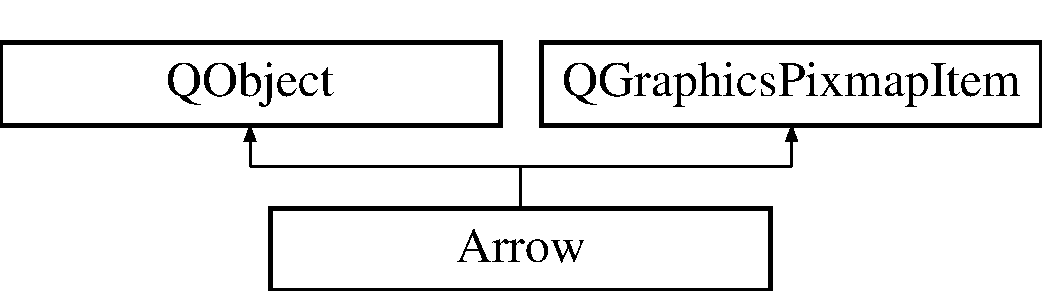
\includegraphics[height=2.000000cm]{classArrow}
\end{center}
\end{figure}
\subsection*{Public Slots}
\begin{DoxyCompactItemize}
\item 
void \hyperlink{classArrow_a0d1bc2ac783f879a9a1c8b86f7eda098}{rotate} ()
\item 
void \hyperlink{classArrow_a48fffc776d41b37884cbfa88c4da9f82}{shoot} ()
\end{DoxyCompactItemize}
\subsection*{Signals}
\begin{DoxyCompactItemize}
\item 
\hypertarget{classArrow_a8e9880f1d08a0bf13f2be7dd9066fea1}{void {\bfseries failure} ()}\label{classArrow_a8e9880f1d08a0bf13f2be7dd9066fea1}

\end{DoxyCompactItemize}
\subsection*{Public Member Functions}
\begin{DoxyCompactItemize}
\item 
\hypertarget{classArrow_a5c5eb1dbfab37de5824bab85b8753a44}{{\bfseries Arrow} (Q\-Object $\ast$parent=nullptr)}\label{classArrow_a5c5eb1dbfab37de5824bab85b8753a44}

\item 
void \hyperlink{classArrow_aa7f35e0a37363c63fb6de0b43f6ca20d}{space\-Pressed} ()
\end{DoxyCompactItemize}
\subsection*{Public Attributes}
\begin{DoxyCompactItemize}
\item 
\hypertarget{classArrow_a5d650c3a3f32e195073714a842cb3ba1}{\hyperlink{classSyringe}{Syringe} $\ast$ {\bfseries syringe}}\label{classArrow_a5d650c3a3f32e195073714a842cb3ba1}

\item 
\hypertarget{classArrow_aa1e4a50a3af88811647d567281d7282f}{Q\-String {\bfseries arrow\-Pic\-Path} = \char`\"{}\-:/game1images/arrow.\-png\char`\"{}}\label{classArrow_aa1e4a50a3af88811647d567281d7282f}

\item 
\hypertarget{classArrow_a432a155342e15549f6a75cf356a5690e}{int {\bfseries direction} = 1}\label{classArrow_a432a155342e15549f6a75cf356a5690e}

\item 
\hypertarget{classArrow_a8d597a253d5a00895021d7bac39e600c}{int {\bfseries rotation\-Degree} = 0}\label{classArrow_a8d597a253d5a00895021d7bac39e600c}

\item 
\hypertarget{classArrow_ae2a16d546410f236d613092aa9f468a8}{int {\bfseries timer\-Rotate\-Speed} = 70}\label{classArrow_ae2a16d546410f236d613092aa9f468a8}

\item 
\hypertarget{classArrow_a5599f9641e83d7eafb79eaf27867aca3}{Q\-Timer $\ast$ {\bfseries timer\-Rotate}}\label{classArrow_a5599f9641e83d7eafb79eaf27867aca3}

\item 
\hypertarget{classArrow_a429a6c14c3ac03613eb705f83cabf25a}{Q\-Timer $\ast$ {\bfseries timer\-Shoot}}\label{classArrow_a429a6c14c3ac03613eb705f83cabf25a}

\end{DoxyCompactItemize}


\subsection{Member Function Documentation}
\hypertarget{classArrow_a0d1bc2ac783f879a9a1c8b86f7eda098}{\index{Arrow@{Arrow}!rotate@{rotate}}
\index{rotate@{rotate}!Arrow@{Arrow}}
\subsubsection[{rotate}]{\setlength{\rightskip}{0pt plus 5cm}void Arrow\-::rotate (
\begin{DoxyParamCaption}
{}
\end{DoxyParamCaption}
)\hspace{0.3cm}{\ttfamily [slot]}}}\label{classArrow_a0d1bc2ac783f879a9a1c8b86f7eda098}
A function to rotate the arrow \hypertarget{classArrow_a48fffc776d41b37884cbfa88c4da9f82}{\index{Arrow@{Arrow}!shoot@{shoot}}
\index{shoot@{shoot}!Arrow@{Arrow}}
\subsubsection[{shoot}]{\setlength{\rightskip}{0pt plus 5cm}void Arrow\-::shoot (
\begin{DoxyParamCaption}
{}
\end{DoxyParamCaption}
)\hspace{0.3cm}{\ttfamily [slot]}}}\label{classArrow_a48fffc776d41b37884cbfa88c4da9f82}
A function to shoot the arrow \hypertarget{classArrow_aa7f35e0a37363c63fb6de0b43f6ca20d}{\index{Arrow@{Arrow}!space\-Pressed@{space\-Pressed}}
\index{space\-Pressed@{space\-Pressed}!Arrow@{Arrow}}
\subsubsection[{space\-Pressed}]{\setlength{\rightskip}{0pt plus 5cm}void Arrow\-::space\-Pressed (
\begin{DoxyParamCaption}
{}
\end{DoxyParamCaption}
)}}\label{classArrow_aa7f35e0a37363c63fb6de0b43f6ca20d}
Creates a new \hyperlink{classSyringe}{Syringe} that gets initalized whenever a space is pressed 

The documentation for this class was generated from the following files\-:\begin{DoxyCompactItemize}
\item 
game1-\/kill-\/covid-\/19/arrow.\-h\item 
game1-\/kill-\/covid-\/19/arrow.\-cpp\end{DoxyCompactItemize}

\hypertarget{classBoard}{\section{Board Class Reference}
\label{classBoard}\index{Board@{Board}}
}
\subsection*{Public Member Functions}
\begin{DoxyCompactItemize}
\item 
void \hyperlink{classBoard_a3eed410fee6da45f4d3fb1135a9e4027}{set\-Score} ()
\item 
\hypertarget{classBoard_aa7d2779562ddb989cfb2c1c1c0257593}{Q\-List$<$ \hyperlink{classPoint}{Point} $>$ {\bfseries get\-Changed\-Tiles} (int player)}\label{classBoard_aa7d2779562ddb989cfb2c1c1c0257593}

\item 
bool \hyperlink{classBoard_aff66d90b976c5723c4ede10596fd4419}{cannot\-Play} (int player)
\end{DoxyCompactItemize}
\subsection*{Public Attributes}
\begin{DoxyCompactItemize}
\item 
\hypertarget{classBoard_ab2156b9c6303a5de76e3c32ba7ebe912}{int {\bfseries count\-Black\-Disks} = 0}\label{classBoard_ab2156b9c6303a5de76e3c32ba7ebe912}

\item 
\hypertarget{classBoard_a6e92b16b78f29fc7b36752deb79279c0}{int {\bfseries count\-White\-Disks} = 0}\label{classBoard_a6e92b16b78f29fc7b36752deb79279c0}

\item 
\hypertarget{classBoard_acf3d60425df85a154a63313b2fb02cfb}{const int {\bfseries player\-White} = -\/1}\label{classBoard_acf3d60425df85a154a63313b2fb02cfb}

\item 
\hypertarget{classBoard_a44b344204eac8428750e0eefe39683ab}{const int {\bfseries player\-Black} = 1}\label{classBoard_a44b344204eac8428750e0eefe39683ab}

\item 
\hypertarget{classBoard_ac7cdacac815beecce696011f51e45953}{int $\ast$$\ast$ {\bfseries gameboard}}\label{classBoard_ac7cdacac815beecce696011f51e45953}

\end{DoxyCompactItemize}


\subsection{Member Function Documentation}
\hypertarget{classBoard_aff66d90b976c5723c4ede10596fd4419}{\index{Board@{Board}!cannot\-Play@{cannot\-Play}}
\index{cannot\-Play@{cannot\-Play}!Board@{Board}}
\subsubsection[{cannot\-Play}]{\setlength{\rightskip}{0pt plus 5cm}bool Board\-::cannot\-Play (
\begin{DoxyParamCaption}
\item[{int}]{player}
\end{DoxyParamCaption}
)}}\label{classBoard_aff66d90b976c5723c4ede10596fd4419}
Checks if a \hyperlink{classUser}{User} or the A\-I can play or not \begin{DoxyReturn}{Returns}
True if they can, false if not 
\end{DoxyReturn}
\hypertarget{classBoard_a3eed410fee6da45f4d3fb1135a9e4027}{\index{Board@{Board}!set\-Score@{set\-Score}}
\index{set\-Score@{set\-Score}!Board@{Board}}
\subsubsection[{set\-Score}]{\setlength{\rightskip}{0pt plus 5cm}void Board\-::set\-Score (
\begin{DoxyParamCaption}
{}
\end{DoxyParamCaption}
)}}\label{classBoard_a3eed410fee6da45f4d3fb1135a9e4027}
Count the number of black and white disks in the board 

The documentation for this class was generated from the following files\-:\begin{DoxyCompactItemize}
\item 
game-\/2-\/reversi/board.\-h\item 
game-\/2-\/reversi/board.\-cpp\end{DoxyCompactItemize}

\hypertarget{classDisk}{\section{Disk Class Reference}
\label{classDisk}\index{Disk@{Disk}}
}
Inheritance diagram for Disk\-:\begin{figure}[H]
\begin{center}
\leavevmode
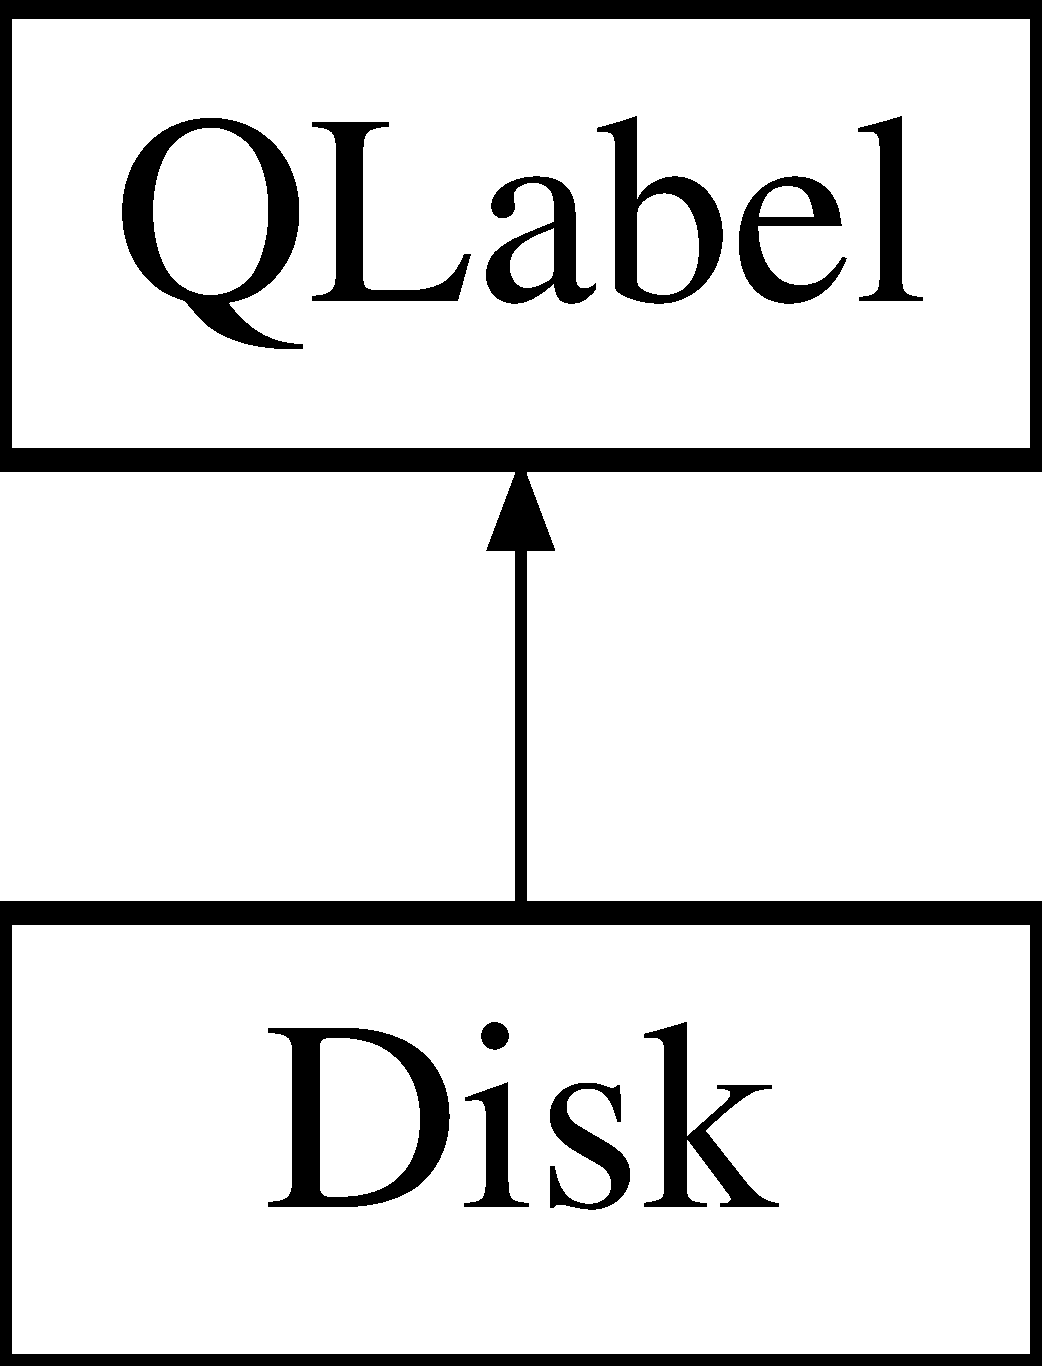
\includegraphics[height=2.000000cm]{classDisk}
\end{center}
\end{figure}
\subsection*{Signals}
\begin{DoxyCompactItemize}
\item 
\hypertarget{classDisk_ada7320e2b6fdc58f1817f4559328234d}{void {\bfseries is\-Clicked} (int x, int y)}\label{classDisk_ada7320e2b6fdc58f1817f4559328234d}

\end{DoxyCompactItemize}
\subsection*{Public Member Functions}
\begin{DoxyCompactItemize}
\item 
\hypertarget{classDisk_ae72358ce74405b34ae94e992c9c99cba}{{\bfseries Disk} (int x, int y, Q\-Widget $\ast$parent=0)}\label{classDisk_ae72358ce74405b34ae94e992c9c99cba}

\end{DoxyCompactItemize}
\subsection*{Protected Member Functions}
\begin{DoxyCompactItemize}
\item 
\hypertarget{classDisk_a4032f507d4b76e07b7698f0f7d35064f}{void {\bfseries mouse\-Press\-Event} (Q\-Mouse\-Event $\ast$event)}\label{classDisk_a4032f507d4b76e07b7698f0f7d35064f}

\end{DoxyCompactItemize}
\subsection*{Protected Attributes}
\begin{DoxyCompactItemize}
\item 
\hypertarget{classDisk_a6d81f44797948383abde236c71d64e24}{int {\bfseries x}}\label{classDisk_a6d81f44797948383abde236c71d64e24}

\item 
\hypertarget{classDisk_a6e79396d7682708ca86ee350af791bc4}{int {\bfseries y}}\label{classDisk_a6e79396d7682708ca86ee350af791bc4}

\end{DoxyCompactItemize}


The documentation for this class was generated from the following files\-:\begin{DoxyCompactItemize}
\item 
game-\/2-\/reversi/disk.\-h\item 
game-\/2-\/reversi/disk.\-cpp\end{DoxyCompactItemize}

\hypertarget{classGame1scene}{\section{Game1scene Class Reference}
\label{classGame1scene}\index{Game1scene@{Game1scene}}
}
Inheritance diagram for Game1scene\-:\begin{figure}[H]
\begin{center}
\leavevmode
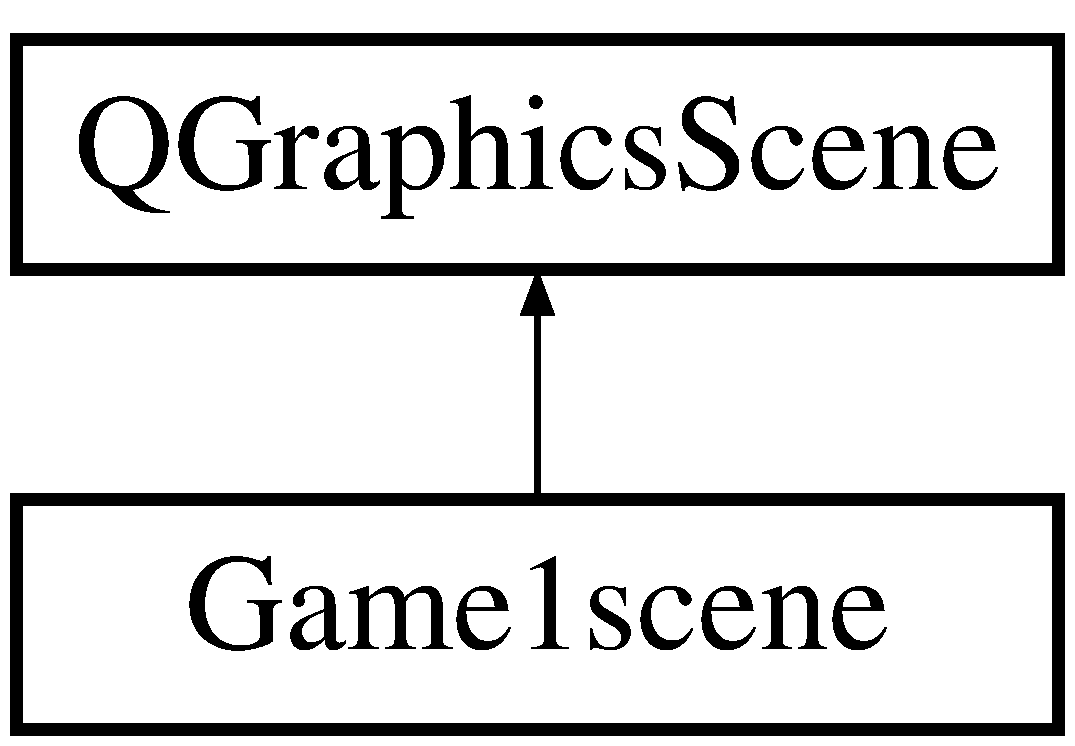
\includegraphics[height=2.000000cm]{classGame1scene}
\end{center}
\end{figure}
\subsection*{Public Slots}
\begin{DoxyCompactItemize}
\item 
void \hyperlink{classGame1scene_aed2bf72aa8fb9698424760590e3eb0de}{start\-Game} ()
\item 
void \hyperlink{classGame1scene_aba975bbe2c5836b193dd7b926b8b0702}{update\-Game\-Name} ()
\item 
void \hyperlink{classGame1scene_a65469907d0aae6863b08ba2ddd1981a0}{update\-Game\-Over} ()
\item 
void \hyperlink{classGame1scene_a3f3f1d903dbdef7ebbc67851fabd4653}{update\-Game\-Won} ()
\item 
void \hyperlink{classGame1scene_a0b4d618af2afa4e519e2deb5e44b865f}{collision\-Virus\-Syring} ()
\item 
void \hyperlink{classGame1scene_abd445be522dcf4d6f6576db9e0f95bee}{user\-Failed} ()
\end{DoxyCompactItemize}
\subsection*{Public Member Functions}
\begin{DoxyCompactItemize}
\item 
\hypertarget{classGame1scene_a92082d74a5921f0f03b24720faefdca9}{void {\bfseries fix\-Widgets} ()}\label{classGame1scene_a92082d74a5921f0f03b24720faefdca9}

\item 
void \hyperlink{classGame1scene_ad0f42592819de78b39f13634fcba633a}{fill\-Scene} ()
\item 
void \hyperlink{classGame1scene_a69cb457788ea97d180888e4448e57ed5}{set\-Score\-Labels} ()
\item 
void \hyperlink{classGame1scene_a9e0a1ce23abc7475ec91d48ec2817c12}{connect\-Buttons} ()
\item 
void \hyperlink{classGame1scene_a9ad6591722ae5f53bef08e27a9fa8f0b}{add\-Circle} ()
\item 
void \hyperlink{classGame1scene_ab4a26256d8a8f57fe62c02952458f297}{display\-Scores} ()
\item 
void \hyperlink{classGame1scene_ae1391e19629f4d73cf7a2c789971b5ff}{add\-Virus} ()
\item 
void \hyperlink{classGame1scene_ac6d3aaa8561d03ae5fd737d4f1472598}{update\-User\-Scores} ()
\item 
void \hyperlink{classGame1scene_a2dcaf7dc9b7d3b490cc5af28d438d543}{increase\-Level} ()
\item 
void \hyperlink{classGame1scene_ac41ffb2804245da3a44a212866a9f574}{user\-Won} ()
\item 
void \hyperlink{classGame1scene_a36fc7dbaa744c866cfb5966c05784d87}{clean\-Page} ()
\end{DoxyCompactItemize}
\subsection*{Public Attributes}
\begin{DoxyCompactItemize}
\item 
\hypertarget{classGame1scene_aab61ae4ec9c39f1b656e0e4e0dd70410}{\hyperlink{classRollingBg}{Rolling\-Bg} $\ast$ {\bfseries rollingbg}}\label{classGame1scene_aab61ae4ec9c39f1b656e0e4e0dd70410}

\item 
\hypertarget{classGame1scene_a2ff871911459d5e25abd0754ebb2a122}{\hyperlink{classSyringe}{Syringe} $\ast$ {\bfseries syringe}}\label{classGame1scene_a2ff871911459d5e25abd0754ebb2a122}

\item 
\hypertarget{classGame1scene_a97e016dd019d53a5d96e80aa6ba49437}{\hyperlink{classArrow}{Arrow} $\ast$ {\bfseries arrow}}\label{classGame1scene_a97e016dd019d53a5d96e80aa6ba49437}

\item 
\hypertarget{classGame1scene_a3be41ab6d1774a4ed4cb52d6d71992ef}{\hyperlink{classVirusLarge}{Virus\-Large} $\ast$ {\bfseries virus\-Large}}\label{classGame1scene_a3be41ab6d1774a4ed4cb52d6d71992ef}

\item 
\hypertarget{classGame1scene_a27d93b7703a0afb753f1c40e60667656}{Q\-Push\-Button $\ast$ {\bfseries home\-Button}}\label{classGame1scene_a27d93b7703a0afb753f1c40e60667656}

\item 
\hypertarget{classGame1scene_afcac285a4f978842c628dddfea9cb694}{Q\-Push\-Button $\ast$ {\bfseries start\-Button}}\label{classGame1scene_afcac285a4f978842c628dddfea9cb694}

\item 
\hypertarget{classGame1scene_a2dc8ee364d557d063dc9176abe3a8a86}{Q\-Graphics\-Pixmap\-Item $\ast$ {\bfseries game\-Name}}\label{classGame1scene_a2dc8ee364d557d063dc9176abe3a8a86}

\item 
\hypertarget{classGame1scene_a71e60cb75619e8cec5edb8b4d155cbc7}{Q\-Graphics\-Pixmap\-Item $\ast$ {\bfseries game\-Over}}\label{classGame1scene_a71e60cb75619e8cec5edb8b4d155cbc7}

\item 
\hypertarget{classGame1scene_a49d0e072e375bb9e43e2e534db60b0c2}{Q\-Graphics\-Pixmap\-Item $\ast$ {\bfseries game\-Won}}\label{classGame1scene_a49d0e072e375bb9e43e2e534db60b0c2}

\item 
\hypertarget{classGame1scene_aa029c0bd0c7bf0a766993ba5f8228c72}{Q\-Graphics\-Pixmap\-Item $\ast$ {\bfseries circle}}\label{classGame1scene_aa029c0bd0c7bf0a766993ba5f8228c72}

\item 
\hypertarget{classGame1scene_a5b73497b52a34341cc3d7eef0184d446}{Q\-Timer $\ast$ {\bfseries game\-Name\-Timer}}\label{classGame1scene_a5b73497b52a34341cc3d7eef0184d446}

\item 
\hypertarget{classGame1scene_a57aecc72a42d6f127628d182bed1b613}{Q\-Timer $\ast$ {\bfseries game\-Over\-Timer}}\label{classGame1scene_a57aecc72a42d6f127628d182bed1b613}

\item 
\hypertarget{classGame1scene_ac08c1b4d9d5fa2f2dc7fda436efa1ace}{Q\-Timer $\ast$ {\bfseries game\-Won\-Timer}}\label{classGame1scene_ac08c1b4d9d5fa2f2dc7fda436efa1ace}

\item 
\hypertarget{classGame1scene_a54e488fa3bc948373489ed07e0be2f05}{int {\bfseries game\-Namey} = 130}\label{classGame1scene_a54e488fa3bc948373489ed07e0be2f05}

\item 
\hypertarget{classGame1scene_ad8d723d4e1db5cad146ff9b71f90baf5}{int {\bfseries game\-Overy} = 130}\label{classGame1scene_ad8d723d4e1db5cad146ff9b71f90baf5}

\item 
\hypertarget{classGame1scene_a6afb0eb5502d469c313d7cbd558e04f9}{int {\bfseries game\-Wony} = 130}\label{classGame1scene_a6afb0eb5502d469c313d7cbd558e04f9}

\item 
\hypertarget{classGame1scene_ae9711bffb3af2e8d3bc95ffdb51ce2a7}{\hyperlink{classUser}{User} $\ast$ {\bfseries cur\-User} = N\-U\-L\-L}\label{classGame1scene_ae9711bffb3af2e8d3bc95ffdb51ce2a7}

\item 
\hypertarget{classGame1scene_a194081c107967a9f825395445b5b2a01}{Q\-Label $\ast$ {\bfseries highscore\-L}}\label{classGame1scene_a194081c107967a9f825395445b5b2a01}

\item 
\hypertarget{classGame1scene_ae5eb0e9d0593cd500e65519b535869c4}{Q\-Label $\ast$ {\bfseries current\-Score\-L}}\label{classGame1scene_ae5eb0e9d0593cd500e65519b535869c4}

\item 
\hypertarget{classGame1scene_a0eb2cbc6c576d2b29a7b175875053059}{Q\-Label $\ast$ {\bfseries score\-History\-L}}\label{classGame1scene_a0eb2cbc6c576d2b29a7b175875053059}

\item 
\hypertarget{classGame1scene_a01a7b045c79aa4a35e162c68cab9d18f}{Q\-Label $\ast$ {\bfseries score\-History}}\label{classGame1scene_a01a7b045c79aa4a35e162c68cab9d18f}

\item 
\hypertarget{classGame1scene_ad8569ca80cc52b6aeca52061d40a07ef}{int {\bfseries highscore} = 0}\label{classGame1scene_ad8569ca80cc52b6aeca52061d40a07ef}

\item 
\hypertarget{classGame1scene_ab5b4b795b2e6ffd778b8643598318670}{int {\bfseries current\-Score} = 0}\label{classGame1scene_ab5b4b795b2e6ffd778b8643598318670}

\item 
\hypertarget{classGame1scene_ad7e822b34258ce63950ec3b4b21f568a}{int {\bfseries count\-Large} = 0}\label{classGame1scene_ad7e822b34258ce63950ec3b4b21f568a}

\item 
\hypertarget{classGame1scene_ad7229285fe01a476de30b721d1048d53}{int {\bfseries count\-Medium} = 0}\label{classGame1scene_ad7229285fe01a476de30b721d1048d53}

\item 
\hypertarget{classGame1scene_abecd4f97ab7cea1988d13796c3bc308f}{int {\bfseries count\-Small} = 0}\label{classGame1scene_abecd4f97ab7cea1988d13796c3bc308f}

\item 
\hypertarget{classGame1scene_a026b32798af9859f763c4499a43ce3fe}{int {\bfseries counter} = 0}\label{classGame1scene_a026b32798af9859f763c4499a43ce3fe}

\item 
\hypertarget{classGame1scene_a0a880df7f091fbc935c8da2767ff52df}{int {\bfseries level\-Speed} = 50}\label{classGame1scene_a0a880df7f091fbc935c8da2767ff52df}

\end{DoxyCompactItemize}


\subsection{Member Function Documentation}
\hypertarget{classGame1scene_a9ad6591722ae5f53bef08e27a9fa8f0b}{\index{Game1scene@{Game1scene}!add\-Circle@{add\-Circle}}
\index{add\-Circle@{add\-Circle}!Game1scene@{Game1scene}}
\subsubsection[{add\-Circle}]{\setlength{\rightskip}{0pt plus 5cm}void Game1scene\-::add\-Circle (
\begin{DoxyParamCaption}
{}
\end{DoxyParamCaption}
)}}\label{classGame1scene_a9ad6591722ae5f53bef08e27a9fa8f0b}
Adds the semi-\/circle that serves as a stand to the arrow \hypertarget{classGame1scene_ae1391e19629f4d73cf7a2c789971b5ff}{\index{Game1scene@{Game1scene}!add\-Virus@{add\-Virus}}
\index{add\-Virus@{add\-Virus}!Game1scene@{Game1scene}}
\subsubsection[{add\-Virus}]{\setlength{\rightskip}{0pt plus 5cm}void Game1scene\-::add\-Virus (
\begin{DoxyParamCaption}
{}
\end{DoxyParamCaption}
)}}\label{classGame1scene_ae1391e19629f4d73cf7a2c789971b5ff}
Creates a new virus and adds it to the game scene \hypertarget{classGame1scene_a36fc7dbaa744c866cfb5966c05784d87}{\index{Game1scene@{Game1scene}!clean\-Page@{clean\-Page}}
\index{clean\-Page@{clean\-Page}!Game1scene@{Game1scene}}
\subsubsection[{clean\-Page}]{\setlength{\rightskip}{0pt plus 5cm}void Game1scene\-::clean\-Page (
\begin{DoxyParamCaption}
{}
\end{DoxyParamCaption}
)}}\label{classGame1scene_a36fc7dbaa744c866cfb5966c05784d87}
Resets the page before admitting a new user \hypertarget{classGame1scene_a0b4d618af2afa4e519e2deb5e44b865f}{\index{Game1scene@{Game1scene}!collision\-Virus\-Syring@{collision\-Virus\-Syring}}
\index{collision\-Virus\-Syring@{collision\-Virus\-Syring}!Game1scene@{Game1scene}}
\subsubsection[{collision\-Virus\-Syring}]{\setlength{\rightskip}{0pt plus 5cm}void Game1scene\-::collision\-Virus\-Syring (
\begin{DoxyParamCaption}
{}
\end{DoxyParamCaption}
)\hspace{0.3cm}{\ttfamily [slot]}}}\label{classGame1scene_a0b4d618af2afa4e519e2deb5e44b865f}
Slot to the collision() signal emitted by the virus\-Large class \hypertarget{classGame1scene_a9e0a1ce23abc7475ec91d48ec2817c12}{\index{Game1scene@{Game1scene}!connect\-Buttons@{connect\-Buttons}}
\index{connect\-Buttons@{connect\-Buttons}!Game1scene@{Game1scene}}
\subsubsection[{connect\-Buttons}]{\setlength{\rightskip}{0pt plus 5cm}void Game1scene\-::connect\-Buttons (
\begin{DoxyParamCaption}
{}
\end{DoxyParamCaption}
)}}\label{classGame1scene_a9e0a1ce23abc7475ec91d48ec2817c12}
Connects all slots and buttons except the virus related ones since we keep creating a new virus everytime. Check \hyperlink{classGame1scene_ae1391e19629f4d73cf7a2c789971b5ff}{Game1scene\-::add\-Virus()} to see the virus related slots. \hypertarget{classGame1scene_ab4a26256d8a8f57fe62c02952458f297}{\index{Game1scene@{Game1scene}!display\-Scores@{display\-Scores}}
\index{display\-Scores@{display\-Scores}!Game1scene@{Game1scene}}
\subsubsection[{display\-Scores}]{\setlength{\rightskip}{0pt plus 5cm}void Game1scene\-::display\-Scores (
\begin{DoxyParamCaption}
{}
\end{DoxyParamCaption}
)}}\label{classGame1scene_ab4a26256d8a8f57fe62c02952458f297}
updates the score labels on the game\-Scene \hypertarget{classGame1scene_ad0f42592819de78b39f13634fcba633a}{\index{Game1scene@{Game1scene}!fill\-Scene@{fill\-Scene}}
\index{fill\-Scene@{fill\-Scene}!Game1scene@{Game1scene}}
\subsubsection[{fill\-Scene}]{\setlength{\rightskip}{0pt plus 5cm}void Game1scene\-::fill\-Scene (
\begin{DoxyParamCaption}
{}
\end{DoxyParamCaption}
)}}\label{classGame1scene_ad0f42592819de78b39f13634fcba633a}
fixes the buttons and adds them to the game Scene \hypertarget{classGame1scene_a2dcaf7dc9b7d3b490cc5af28d438d543}{\index{Game1scene@{Game1scene}!increase\-Level@{increase\-Level}}
\index{increase\-Level@{increase\-Level}!Game1scene@{Game1scene}}
\subsubsection[{increase\-Level}]{\setlength{\rightskip}{0pt plus 5cm}void Game1scene\-::increase\-Level (
\begin{DoxyParamCaption}
{}
\end{DoxyParamCaption}
)}}\label{classGame1scene_a2dcaf7dc9b7d3b490cc5af28d438d543}
Called whenever the user hits 5 viruses. increases the speed of rotation of arrows as well as the speed of the viruses (level\-Speed) and rolling background \hypertarget{classGame1scene_a69cb457788ea97d180888e4448e57ed5}{\index{Game1scene@{Game1scene}!set\-Score\-Labels@{set\-Score\-Labels}}
\index{set\-Score\-Labels@{set\-Score\-Labels}!Game1scene@{Game1scene}}
\subsubsection[{set\-Score\-Labels}]{\setlength{\rightskip}{0pt plus 5cm}void Game1scene\-::set\-Score\-Labels (
\begin{DoxyParamCaption}
{}
\end{DoxyParamCaption}
)}}\label{classGame1scene_a69cb457788ea97d180888e4448e57ed5}
Fixes the score labels and adds them to the scene \hypertarget{classGame1scene_aed2bf72aa8fb9698424760590e3eb0de}{\index{Game1scene@{Game1scene}!start\-Game@{start\-Game}}
\index{start\-Game@{start\-Game}!Game1scene@{Game1scene}}
\subsubsection[{start\-Game}]{\setlength{\rightskip}{0pt plus 5cm}void Game1scene\-::start\-Game (
\begin{DoxyParamCaption}
{}
\end{DoxyParamCaption}
)\hspace{0.3cm}{\ttfamily [slot]}}}\label{classGame1scene_aed2bf72aa8fb9698424760590e3eb0de}
Resets the current scores and starts a new game \hypertarget{classGame1scene_aba975bbe2c5836b193dd7b926b8b0702}{\index{Game1scene@{Game1scene}!update\-Game\-Name@{update\-Game\-Name}}
\index{update\-Game\-Name@{update\-Game\-Name}!Game1scene@{Game1scene}}
\subsubsection[{update\-Game\-Name}]{\setlength{\rightskip}{0pt plus 5cm}void Game1scene\-::update\-Game\-Name (
\begin{DoxyParamCaption}
{}
\end{DoxyParamCaption}
)\hspace{0.3cm}{\ttfamily [slot]}}}\label{classGame1scene_aba975bbe2c5836b193dd7b926b8b0702}
Makes game\-Name label move up and down \hypertarget{classGame1scene_a65469907d0aae6863b08ba2ddd1981a0}{\index{Game1scene@{Game1scene}!update\-Game\-Over@{update\-Game\-Over}}
\index{update\-Game\-Over@{update\-Game\-Over}!Game1scene@{Game1scene}}
\subsubsection[{update\-Game\-Over}]{\setlength{\rightskip}{0pt plus 5cm}void Game1scene\-::update\-Game\-Over (
\begin{DoxyParamCaption}
{}
\end{DoxyParamCaption}
)\hspace{0.3cm}{\ttfamily [slot]}}}\label{classGame1scene_a65469907d0aae6863b08ba2ddd1981a0}
Makes game\-Over label move up and down \hypertarget{classGame1scene_a3f3f1d903dbdef7ebbc67851fabd4653}{\index{Game1scene@{Game1scene}!update\-Game\-Won@{update\-Game\-Won}}
\index{update\-Game\-Won@{update\-Game\-Won}!Game1scene@{Game1scene}}
\subsubsection[{update\-Game\-Won}]{\setlength{\rightskip}{0pt plus 5cm}void Game1scene\-::update\-Game\-Won (
\begin{DoxyParamCaption}
{}
\end{DoxyParamCaption}
)\hspace{0.3cm}{\ttfamily [slot]}}}\label{classGame1scene_a3f3f1d903dbdef7ebbc67851fabd4653}
Makes game\-Won label move up and down \hypertarget{classGame1scene_ac6d3aaa8561d03ae5fd737d4f1472598}{\index{Game1scene@{Game1scene}!update\-User\-Scores@{update\-User\-Scores}}
\index{update\-User\-Scores@{update\-User\-Scores}!Game1scene@{Game1scene}}
\subsubsection[{update\-User\-Scores}]{\setlength{\rightskip}{0pt plus 5cm}void Game1scene\-::update\-User\-Scores (
\begin{DoxyParamCaption}
{}
\end{DoxyParamCaption}
)}}\label{classGame1scene_ac6d3aaa8561d03ae5fd737d4f1472598}
Edits the current \hyperlink{classUser}{User}'s vector of game1 scores as well as his highscore \hypertarget{classGame1scene_abd445be522dcf4d6f6576db9e0f95bee}{\index{Game1scene@{Game1scene}!user\-Failed@{user\-Failed}}
\index{user\-Failed@{user\-Failed}!Game1scene@{Game1scene}}
\subsubsection[{user\-Failed}]{\setlength{\rightskip}{0pt plus 5cm}void Game1scene\-::user\-Failed (
\begin{DoxyParamCaption}
{}
\end{DoxyParamCaption}
)\hspace{0.3cm}{\ttfamily [slot]}}}\label{classGame1scene_abd445be522dcf4d6f6576db9e0f95bee}
Whenever the arrow goes out of bound or when a virus leaves the boundary without being hit, this function receives the failure() signal and ends the current game \hypertarget{classGame1scene_ac41ffb2804245da3a44a212866a9f574}{\index{Game1scene@{Game1scene}!user\-Won@{user\-Won}}
\index{user\-Won@{user\-Won}!Game1scene@{Game1scene}}
\subsubsection[{user\-Won}]{\setlength{\rightskip}{0pt plus 5cm}void Game1scene\-::user\-Won (
\begin{DoxyParamCaption}
{}
\end{DoxyParamCaption}
)}}\label{classGame1scene_ac41ffb2804245da3a44a212866a9f574}
whenever the user reaches a score $>$= 150 this function signals that the user wins and ends the current game 

The documentation for this class was generated from the following files\-:\begin{DoxyCompactItemize}
\item 
game1-\/kill-\/covid-\/19/game1scene.\-h\item 
game1-\/kill-\/covid-\/19/game1scene.\-cpp\end{DoxyCompactItemize}

\hypertarget{classGame2scene}{\section{Game2scene Class Reference}
\label{classGame2scene}\index{Game2scene@{Game2scene}}
}
Inheritance diagram for Game2scene\-:\begin{figure}[H]
\begin{center}
\leavevmode
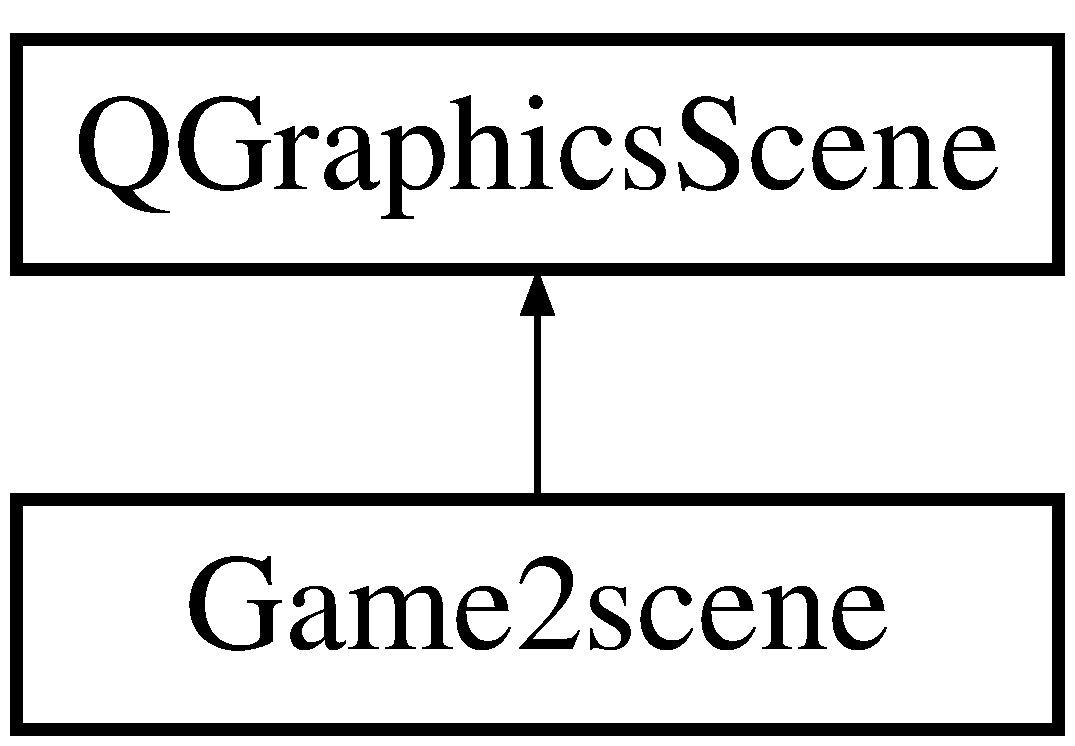
\includegraphics[height=2.000000cm]{classGame2scene}
\end{center}
\end{figure}
\subsection*{Public Slots}
\begin{DoxyCompactItemize}
\item 
void \hyperlink{classGame2scene_a2721090205eb61711f1e0395984f93c0}{cell\-Clicked} ()
\item 
void \hyperlink{classGame2scene_ab2260f4670232d77bf1f24b2bc98c785}{change\-Turn} ()
\item 
void \hyperlink{classGame2scene_a0d79d8188020496d4af3bc67b5a56020}{restart\-Game} ()
\end{DoxyCompactItemize}
\subsection*{Public Member Functions}
\begin{DoxyCompactItemize}
\item 
void \hyperlink{classGame2scene_a18ee83d97ffb17df3d554f01c113ecd9}{start\-Game} ()
\item 
void \hyperlink{classGame2scene_a97e66e2641f6c77daba82b99c50056ac}{change\-To\-Player} ()
\item 
bool \hyperlink{classGame2scene_a2d603c8abf5eb9789b8fd160f1a339b2}{legal\-Moves\-Check} ()
\item 
void \hyperlink{classGame2scene_ad56cf11d5f9cf0159286885b8c3886f2}{update\-Board} ()
\item 
void \hyperlink{classGame2scene_aaedfb29d950f472dd031869e1974837a}{game\-Over} ()
\item 
void \hyperlink{classGame2scene_a844342045953eba83bac963b282e55a5}{fill\-Scene} ()
\item 
void \hyperlink{classGame2scene_af8d371d3e0d151a5535bae0e735c7dc3}{fill\-Scene\-Helper} (Q\-Label $\ast$label, int font\-Size)
\item 
void \hyperlink{classGame2scene_a6968b1e0acbc0054c43014b7a38400fd}{update\-User\-Scores} ()
\item 
void \hyperlink{classGame2scene_ae9990344a0346f2b594e4476fdb5e312}{clean\-Page} ()
\end{DoxyCompactItemize}
\subsection*{Public Attributes}
\begin{DoxyCompactItemize}
\item 
\hypertarget{classGame2scene_ad29d2d44e8aed6f12220d80b39982376}{\hyperlink{classUser}{User} $\ast$ {\bfseries cur\-User} = N\-U\-L\-L}\label{classGame2scene_ad29d2d44e8aed6f12220d80b39982376}

\item 
\hypertarget{classGame2scene_a86b35242a3f532c24763bb83f2f586ea}{int {\bfseries highscore} = 0}\label{classGame2scene_a86b35242a3f532c24763bb83f2f586ea}

\item 
\hypertarget{classGame2scene_a3605ef4645d5cf2048a3ea53ff8f19fa}{\hyperlink{classBoard}{Board} $\ast$ {\bfseries board}}\label{classGame2scene_a3605ef4645d5cf2048a3ea53ff8f19fa}

\item 
\hypertarget{classGame2scene_a49d8afe92b6338c8adc1309546670e79}{Q\-Timer $\ast$ {\bfseries timer}}\label{classGame2scene_a49d8afe92b6338c8adc1309546670e79}

\item 
\hypertarget{classGame2scene_a71f9e685aa7a31054d49772c49470d06}{Q\-Graphics\-Pixmap\-Item $\ast$ {\bfseries board\-Picture}}\label{classGame2scene_a71f9e685aa7a31054d49772c49470d06}

\item 
\hypertarget{classGame2scene_ab4d95cabb6503aa6230209b87e0d8c44}{Q\-Graphics\-Pixmap\-Item $\ast$ {\bfseries game\-Name\-Picture}}\label{classGame2scene_ab4d95cabb6503aa6230209b87e0d8c44}

\item 
\hypertarget{classGame2scene_a8a3827271508af74fd6d8afc1a8d5e25}{Q\-String {\bfseries white\-Image} = \char`\"{}\-:/game2images/White\-Disk.\-png\char`\"{}}\label{classGame2scene_a8a3827271508af74fd6d8afc1a8d5e25}

\item 
\hypertarget{classGame2scene_a0c958503508709dc05815acc6b7465e8}{Q\-String {\bfseries black\-I\-Mage} = \char`\"{}\-:/game2images/Black\-Disk.\-png\char`\"{}}\label{classGame2scene_a0c958503508709dc05815acc6b7465e8}

\item 
\hypertarget{classGame2scene_a67ab6963073d76ed6d8d065fd1014e8c}{Q\-Label $\ast$ {\bfseries row}}\label{classGame2scene_a67ab6963073d76ed6d8d065fd1014e8c}

\item 
\hypertarget{classGame2scene_aa9250f1765d7c6d4f10cd31735440bbe}{Q\-Label $\ast$ {\bfseries column}}\label{classGame2scene_aa9250f1765d7c6d4f10cd31735440bbe}

\item 
\hypertarget{classGame2scene_a2e55d1c496f520b7b947d6f172b78936}{Q\-Label $\ast$ {\bfseries final\-Score}}\label{classGame2scene_a2e55d1c496f520b7b947d6f172b78936}

\item 
\hypertarget{classGame2scene_a64398d57b719a9f0988644d5f216dc1f}{Q\-Label $\ast$ {\bfseries game\-Name}}\label{classGame2scene_a64398d57b719a9f0988644d5f216dc1f}

\item 
\hypertarget{classGame2scene_a679ac7cdbe944211fd6e691d2586ba0a}{Q\-Label $\ast$ {\bfseries row\-Numbers}}\label{classGame2scene_a679ac7cdbe944211fd6e691d2586ba0a}

\item 
\hypertarget{classGame2scene_a6105168ba444e82a4245bfcbf07d1e21}{Q\-Label $\ast$ {\bfseries col\-Numbers}}\label{classGame2scene_a6105168ba444e82a4245bfcbf07d1e21}

\item 
\hypertarget{classGame2scene_a49f2bb5c4e1e4660506fbfec5a5c6c1d}{Q\-Line\-Edit $\ast$ {\bfseries row\-Edit}}\label{classGame2scene_a49f2bb5c4e1e4660506fbfec5a5c6c1d}

\item 
\hypertarget{classGame2scene_ae0c7376c62ad8fb669bc3a6fedf429a4}{Q\-Line\-Edit $\ast$ {\bfseries column\-Edit}}\label{classGame2scene_ae0c7376c62ad8fb669bc3a6fedf429a4}

\item 
\hypertarget{classGame2scene_a6a69bd47926bf33845f59b6e08a2d42d}{Q\-Push\-Button $\ast$ {\bfseries enter\-Move}}\label{classGame2scene_a6a69bd47926bf33845f59b6e08a2d42d}

\item 
\hypertarget{classGame2scene_a31108de508257e90666bc180f9d4cc01}{Q\-Push\-Button $\ast$ {\bfseries home\-Button}}\label{classGame2scene_a31108de508257e90666bc180f9d4cc01}

\item 
\hypertarget{classGame2scene_a1ab905edfb95dcc9385ab11951c9e564}{Q\-Push\-Button $\ast$ {\bfseries restart\-Button}}\label{classGame2scene_a1ab905edfb95dcc9385ab11951c9e564}

\item 
\hypertarget{classGame2scene_a97b9cd4f181babf7731cab15b59a61ac}{Q\-Graphics\-Pixmap\-Item $\ast$$\ast$$\ast$ {\bfseries board\-Game}}\label{classGame2scene_a97b9cd4f181babf7731cab15b59a61ac}

\item 
\hypertarget{classGame2scene_ae50096081fc348256d987f71f79c0487}{int {\bfseries game\-Status} = -\/1}\label{classGame2scene_ae50096081fc348256d987f71f79c0487}

\end{DoxyCompactItemize}


\subsection{Member Function Documentation}
\hypertarget{classGame2scene_a2721090205eb61711f1e0395984f93c0}{\index{Game2scene@{Game2scene}!cell\-Clicked@{cell\-Clicked}}
\index{cell\-Clicked@{cell\-Clicked}!Game2scene@{Game2scene}}
\subsubsection[{cell\-Clicked}]{\setlength{\rightskip}{0pt plus 5cm}void Game2scene\-::cell\-Clicked (
\begin{DoxyParamCaption}
{}
\end{DoxyParamCaption}
)\hspace{0.3cm}{\ttfamily [slot]}}}\label{classGame2scene_a2721090205eb61711f1e0395984f93c0}
A function that updates the board whenever an input from the user is given. \hypertarget{classGame2scene_a97e66e2641f6c77daba82b99c50056ac}{\index{Game2scene@{Game2scene}!change\-To\-Player@{change\-To\-Player}}
\index{change\-To\-Player@{change\-To\-Player}!Game2scene@{Game2scene}}
\subsubsection[{change\-To\-Player}]{\setlength{\rightskip}{0pt plus 5cm}void Game2scene\-::change\-To\-Player (
\begin{DoxyParamCaption}
{}
\end{DoxyParamCaption}
)}}\label{classGame2scene_a97e66e2641f6c77daba82b99c50056ac}
A function used to do the logic whenever we change the player's turn \hypertarget{classGame2scene_ab2260f4670232d77bf1f24b2bc98c785}{\index{Game2scene@{Game2scene}!change\-Turn@{change\-Turn}}
\index{change\-Turn@{change\-Turn}!Game2scene@{Game2scene}}
\subsubsection[{change\-Turn}]{\setlength{\rightskip}{0pt plus 5cm}void Game2scene\-::change\-Turn (
\begin{DoxyParamCaption}
{}
\end{DoxyParamCaption}
)\hspace{0.3cm}{\ttfamily [slot]}}}\label{classGame2scene_ab2260f4670232d77bf1f24b2bc98c785}
A function used to change turns between players \hypertarget{classGame2scene_ae9990344a0346f2b594e4476fdb5e312}{\index{Game2scene@{Game2scene}!clean\-Page@{clean\-Page}}
\index{clean\-Page@{clean\-Page}!Game2scene@{Game2scene}}
\subsubsection[{clean\-Page}]{\setlength{\rightskip}{0pt plus 5cm}void Game2scene\-::clean\-Page (
\begin{DoxyParamCaption}
{}
\end{DoxyParamCaption}
)}}\label{classGame2scene_ae9990344a0346f2b594e4476fdb5e312}
A function that cleans the page and remove items from the board when a user chooses to go back to the home page \hypertarget{classGame2scene_a844342045953eba83bac963b282e55a5}{\index{Game2scene@{Game2scene}!fill\-Scene@{fill\-Scene}}
\index{fill\-Scene@{fill\-Scene}!Game2scene@{Game2scene}}
\subsubsection[{fill\-Scene}]{\setlength{\rightskip}{0pt plus 5cm}void Game2scene\-::fill\-Scene (
\begin{DoxyParamCaption}
{}
\end{DoxyParamCaption}
)}}\label{classGame2scene_a844342045953eba83bac963b282e55a5}
A function to fill the scene \hypertarget{classGame2scene_af8d371d3e0d151a5535bae0e735c7dc3}{\index{Game2scene@{Game2scene}!fill\-Scene\-Helper@{fill\-Scene\-Helper}}
\index{fill\-Scene\-Helper@{fill\-Scene\-Helper}!Game2scene@{Game2scene}}
\subsubsection[{fill\-Scene\-Helper}]{\setlength{\rightskip}{0pt plus 5cm}void Game2scene\-::fill\-Scene\-Helper (
\begin{DoxyParamCaption}
\item[{Q\-Label $\ast$}]{label, }
\item[{int}]{font\-Size}
\end{DoxyParamCaption}
)}}\label{classGame2scene_af8d371d3e0d151a5535bae0e735c7dc3}
A helper function to fill the Scene \hypertarget{classGame2scene_aaedfb29d950f472dd031869e1974837a}{\index{Game2scene@{Game2scene}!game\-Over@{game\-Over}}
\index{game\-Over@{game\-Over}!Game2scene@{Game2scene}}
\subsubsection[{game\-Over}]{\setlength{\rightskip}{0pt plus 5cm}void Game2scene\-::game\-Over (
\begin{DoxyParamCaption}
{}
\end{DoxyParamCaption}
)}}\label{classGame2scene_aaedfb29d950f472dd031869e1974837a}
A function used to do the logic when a game finishes. \hypertarget{classGame2scene_a2d603c8abf5eb9789b8fd160f1a339b2}{\index{Game2scene@{Game2scene}!legal\-Moves\-Check@{legal\-Moves\-Check}}
\index{legal\-Moves\-Check@{legal\-Moves\-Check}!Game2scene@{Game2scene}}
\subsubsection[{legal\-Moves\-Check}]{\setlength{\rightskip}{0pt plus 5cm}bool Game2scene\-::legal\-Moves\-Check (
\begin{DoxyParamCaption}
{}
\end{DoxyParamCaption}
)}}\label{classGame2scene_a2d603c8abf5eb9789b8fd160f1a339b2}
Checks if the play or A\-I can make a move \begin{DoxyReturn}{Returns}
True if they can, false if not 
\end{DoxyReturn}
\hypertarget{classGame2scene_a0d79d8188020496d4af3bc67b5a56020}{\index{Game2scene@{Game2scene}!restart\-Game@{restart\-Game}}
\index{restart\-Game@{restart\-Game}!Game2scene@{Game2scene}}
\subsubsection[{restart\-Game}]{\setlength{\rightskip}{0pt plus 5cm}void Game2scene\-::restart\-Game (
\begin{DoxyParamCaption}
{}
\end{DoxyParamCaption}
)\hspace{0.3cm}{\ttfamily [slot]}}}\label{classGame2scene_a0d79d8188020496d4af3bc67b5a56020}
A function used to restart the game whenever the button is clicked \hypertarget{classGame2scene_a18ee83d97ffb17df3d554f01c113ecd9}{\index{Game2scene@{Game2scene}!start\-Game@{start\-Game}}
\index{start\-Game@{start\-Game}!Game2scene@{Game2scene}}
\subsubsection[{start\-Game}]{\setlength{\rightskip}{0pt plus 5cm}void Game2scene\-::start\-Game (
\begin{DoxyParamCaption}
{}
\end{DoxyParamCaption}
)}}\label{classGame2scene_a18ee83d97ffb17df3d554f01c113ecd9}
A function Used by the constructor to start the game and initalize the board and images \hypertarget{classGame2scene_ad56cf11d5f9cf0159286885b8c3886f2}{\index{Game2scene@{Game2scene}!update\-Board@{update\-Board}}
\index{update\-Board@{update\-Board}!Game2scene@{Game2scene}}
\subsubsection[{update\-Board}]{\setlength{\rightskip}{0pt plus 5cm}void Game2scene\-::update\-Board (
\begin{DoxyParamCaption}
{}
\end{DoxyParamCaption}
)}}\label{classGame2scene_ad56cf11d5f9cf0159286885b8c3886f2}
Updates the board's pixmaps whenever a turn is finished. \hypertarget{classGame2scene_a6968b1e0acbc0054c43014b7a38400fd}{\index{Game2scene@{Game2scene}!update\-User\-Scores@{update\-User\-Scores}}
\index{update\-User\-Scores@{update\-User\-Scores}!Game2scene@{Game2scene}}
\subsubsection[{update\-User\-Scores}]{\setlength{\rightskip}{0pt plus 5cm}void Game2scene\-::update\-User\-Scores (
\begin{DoxyParamCaption}
{}
\end{DoxyParamCaption}
)}}\label{classGame2scene_a6968b1e0acbc0054c43014b7a38400fd}
Edits the current \hyperlink{classUser}{User}'s vector of game2 scores as well as his highscore 

The documentation for this class was generated from the following files\-:\begin{DoxyCompactItemize}
\item 
game-\/2-\/reversi/game2scene.\-h\item 
game-\/2-\/reversi/game2scene.\-cpp\end{DoxyCompactItemize}

\hypertarget{classJson}{\section{Json Class Reference}
\label{classJson}\index{Json@{Json}}
}
\subsection*{Public Member Functions}
\begin{DoxyCompactItemize}
\item 
Q\-Json\-Document \hyperlink{classJson_a8f60a3a23f11ac93003d1c3e0e069dde}{get\-Json\-Document} ()
\begin{DoxyCompactList}\small\item\em Gets the Json\-Document of the file path. \end{DoxyCompactList}\item 
void \hyperlink{classJson_afe466a1ce0a4f747a366029db26ee9a3}{append\-To\-User\-Document} (Q\-Json\-Object user)
\item 
void \hyperlink{classJson_a21ad90aadf8443aab3f4a60288ee100a}{update\-User\-Scores} (Q\-String username, Q\-Vector$<$ int $>$ game\-Scores, int highscore, int game\-Number)
\item 
Q\-Json\-Object \hyperlink{classJson_a515ca3c26feb507e7da11cdf61ec77cd}{check\-User} (Q\-Json\-Array \&users\-Array, Q\-String \&username, Q\-String \&password)
\item 
Q\-Json\-Value \hyperlink{classJson_a89ce8478fc9da72e964e6aef97604ae3}{Encode\-Image} (const Q\-Pixmap \&p)
\item 
\hypertarget{classJson_a2586512a930bc5631183cf2b722e91eb}{Q\-Pixmap {\bfseries Decode\-Image} (Q\-Json\-Value val)}\label{classJson_a2586512a930bc5631183cf2b722e91eb}

\end{DoxyCompactItemize}
\subsection*{Public Attributes}
\begin{DoxyCompactItemize}
\item 
\hypertarget{classJson_ad637dea3aa5aa005b0b21af4bbc59328}{Q\-String {\bfseries file\-Path} = \char`\"{}/home/eece435l/Desktop/435\-L/project-\/eece435l-\/game-\/center/\-J\-S\-O\-N/users.\-json\char`\"{}}\label{classJson_ad637dea3aa5aa005b0b21af4bbc59328}

\item 
\hypertarget{classJson_ac414a8d0e58941fbe840808c32fb1879}{\hyperlink{classUtil}{Util} {\bfseries util}}\label{classJson_ac414a8d0e58941fbe840808c32fb1879}

\end{DoxyCompactItemize}


\subsection{Member Function Documentation}
\hypertarget{classJson_afe466a1ce0a4f747a366029db26ee9a3}{\index{Json@{Json}!append\-To\-User\-Document@{append\-To\-User\-Document}}
\index{append\-To\-User\-Document@{append\-To\-User\-Document}!Json@{Json}}
\subsubsection[{append\-To\-User\-Document}]{\setlength{\rightskip}{0pt plus 5cm}void Json\-::append\-To\-User\-Document (
\begin{DoxyParamCaption}
\item[{Q\-Json\-Object}]{user}
\end{DoxyParamCaption}
)}}\label{classJson_afe466a1ce0a4f747a366029db26ee9a3}
Takes a newly created user and appends it to the users.\-json document \hypertarget{classJson_a515ca3c26feb507e7da11cdf61ec77cd}{\index{Json@{Json}!check\-User@{check\-User}}
\index{check\-User@{check\-User}!Json@{Json}}
\subsubsection[{check\-User}]{\setlength{\rightskip}{0pt plus 5cm}Q\-Json\-Object Json\-::check\-User (
\begin{DoxyParamCaption}
\item[{Q\-Json\-Array \&}]{users\-Array, }
\item[{Q\-String \&}]{username, }
\item[{Q\-String \&}]{password}
\end{DoxyParamCaption}
)}}\label{classJson_a515ca3c26feb507e7da11cdf61ec77cd}
Checks if a user who attempted to login has already signed up before \begin{DoxyReturn}{Returns}
If the login was successful, returns the user as a Q\-Json\-Object.\-Else returns an empty Q\-J\-Son\-Object 
\end{DoxyReturn}
\hypertarget{classJson_a89ce8478fc9da72e964e6aef97604ae3}{\index{Json@{Json}!Encode\-Image@{Encode\-Image}}
\index{Encode\-Image@{Encode\-Image}!Json@{Json}}
\subsubsection[{Encode\-Image}]{\setlength{\rightskip}{0pt plus 5cm}Q\-Json\-Value Json\-::\-Encode\-Image (
\begin{DoxyParamCaption}
\item[{const Q\-Pixmap \&}]{p}
\end{DoxyParamCaption}
)}}\label{classJson_a89ce8478fc9da72e964e6aef97604ae3}
Takes a picture, encodes it, and returns the corresponding hashed Q\-Json\-Value \begin{DoxyReturn}{Returns}
Q\-Json\-Value for the encoded image 
\end{DoxyReturn}
\hypertarget{classJson_a8f60a3a23f11ac93003d1c3e0e069dde}{\index{Json@{Json}!get\-Json\-Document@{get\-Json\-Document}}
\index{get\-Json\-Document@{get\-Json\-Document}!Json@{Json}}
\subsubsection[{get\-Json\-Document}]{\setlength{\rightskip}{0pt plus 5cm}Q\-Json\-Document Json\-::get\-Json\-Document (
\begin{DoxyParamCaption}
{}
\end{DoxyParamCaption}
)}}\label{classJson_a8f60a3a23f11ac93003d1c3e0e069dde}


Gets the Json\-Document of the file path. 

\begin{DoxyReturn}{Returns}
Q\-Json\-Document of the file path 
\end{DoxyReturn}
\hypertarget{classJson_a21ad90aadf8443aab3f4a60288ee100a}{\index{Json@{Json}!update\-User\-Scores@{update\-User\-Scores}}
\index{update\-User\-Scores@{update\-User\-Scores}!Json@{Json}}
\subsubsection[{update\-User\-Scores}]{\setlength{\rightskip}{0pt plus 5cm}void Json\-::update\-User\-Scores (
\begin{DoxyParamCaption}
\item[{Q\-String}]{username, }
\item[{Q\-Vector$<$ int $>$}]{game\-Scores, }
\item[{int}]{highscore, }
\item[{int}]{game\-Number}
\end{DoxyParamCaption}
)}}\label{classJson_a21ad90aadf8443aab3f4a60288ee100a}
Update the \hyperlink{classUser}{User} Scores in the \hyperlink{classJson}{Json} object of the \hyperlink{classUser}{User} 

The documentation for this class was generated from the following files\-:\begin{DoxyCompactItemize}
\item 
accounts-\/and-\/framework/json.\-h\item 
accounts-\/and-\/framework/json.\-cpp\end{DoxyCompactItemize}

\hypertarget{classLine}{\section{Line Class Reference}
\label{classLine}\index{Line@{Line}}
}
\subsection*{Public Member Functions}
\begin{DoxyCompactItemize}
\item 
Q\-List$<$ \hyperlink{classPoint}{Point} $>$ \hyperlink{classLine_a91d2b5b17efce31863c4ba2545cc3917}{get\-Changed\-Tiles} ()
\item 
Q\-List$<$ \hyperlink{classPoint}{Point} $>$ \hyperlink{classLine_ac7cf1abd6bdabad3ae7589c716920af6}{check\-Line} (\hyperlink{classPoint}{Point} pattern)
\item 
\hypertarget{classLine_ad1cf45f33ea7256560fe6ce4fc2d1eb2}{{\bfseries Line} (int disk\-Color, \hyperlink{classPoint}{Point} point, int $\ast$$\ast$board)}\label{classLine_ad1cf45f33ea7256560fe6ce4fc2d1eb2}

\end{DoxyCompactItemize}
\subsection*{Public Attributes}
\begin{DoxyCompactItemize}
\item 
\hypertarget{classLine_a35580843d14864454cddd16d7806049c}{int {\bfseries disk\-Color}}\label{classLine_a35580843d14864454cddd16d7806049c}

\item 
\hypertarget{classLine_adaf06f2ff9499915e340b615ecade2a7}{\hyperlink{classPoint}{Point} {\bfseries point}}\label{classLine_adaf06f2ff9499915e340b615ecade2a7}

\item 
\hypertarget{classLine_ac9918112d0314311e32c819cdc100ebf}{int $\ast$$\ast$ {\bfseries boardgame}}\label{classLine_ac9918112d0314311e32c819cdc100ebf}

\end{DoxyCompactItemize}


\subsection{Member Function Documentation}
\hypertarget{classLine_ac7cf1abd6bdabad3ae7589c716920af6}{\index{Line@{Line}!check\-Line@{check\-Line}}
\index{check\-Line@{check\-Line}!Line@{Line}}
\subsubsection[{check\-Line}]{\setlength{\rightskip}{0pt plus 5cm}Q\-List$<$ {\bf Point} $>$ Line\-::check\-Line (
\begin{DoxyParamCaption}
\item[{{\bf Point}}]{pattern}
\end{DoxyParamCaption}
)}}\label{classLine_ac7cf1abd6bdabad3ae7589c716920af6}
A function used by get\-Changed\-Tiles to see whether a line is affected by the point \begin{DoxyReturn}{Returns}
If it is affected, it returns a list of all points affected. If not, it just returns an empty list 
\end{DoxyReturn}
\hypertarget{classLine_a91d2b5b17efce31863c4ba2545cc3917}{\index{Line@{Line}!get\-Changed\-Tiles@{get\-Changed\-Tiles}}
\index{get\-Changed\-Tiles@{get\-Changed\-Tiles}!Line@{Line}}
\subsubsection[{get\-Changed\-Tiles}]{\setlength{\rightskip}{0pt plus 5cm}Q\-List$<$ {\bf Point} $>$ Line\-::get\-Changed\-Tiles (
\begin{DoxyParamCaption}
{}
\end{DoxyParamCaption}
)}}\label{classLine_a91d2b5b17efce31863c4ba2545cc3917}
A function that get all the changed tiles that are affected by choosing the point attribute \begin{DoxyReturn}{Returns}
A list of all changed points on the board 
\end{DoxyReturn}


The documentation for this class was generated from the following files\-:\begin{DoxyCompactItemize}
\item 
game-\/2-\/reversi/line.\-h\item 
game-\/2-\/reversi/line.\-cpp\end{DoxyCompactItemize}

\hypertarget{classLoginPage}{\section{Login\-Page Class Reference}
\label{classLoginPage}\index{Login\-Page@{Login\-Page}}
}
Inheritance diagram for Login\-Page\-:\begin{figure}[H]
\begin{center}
\leavevmode
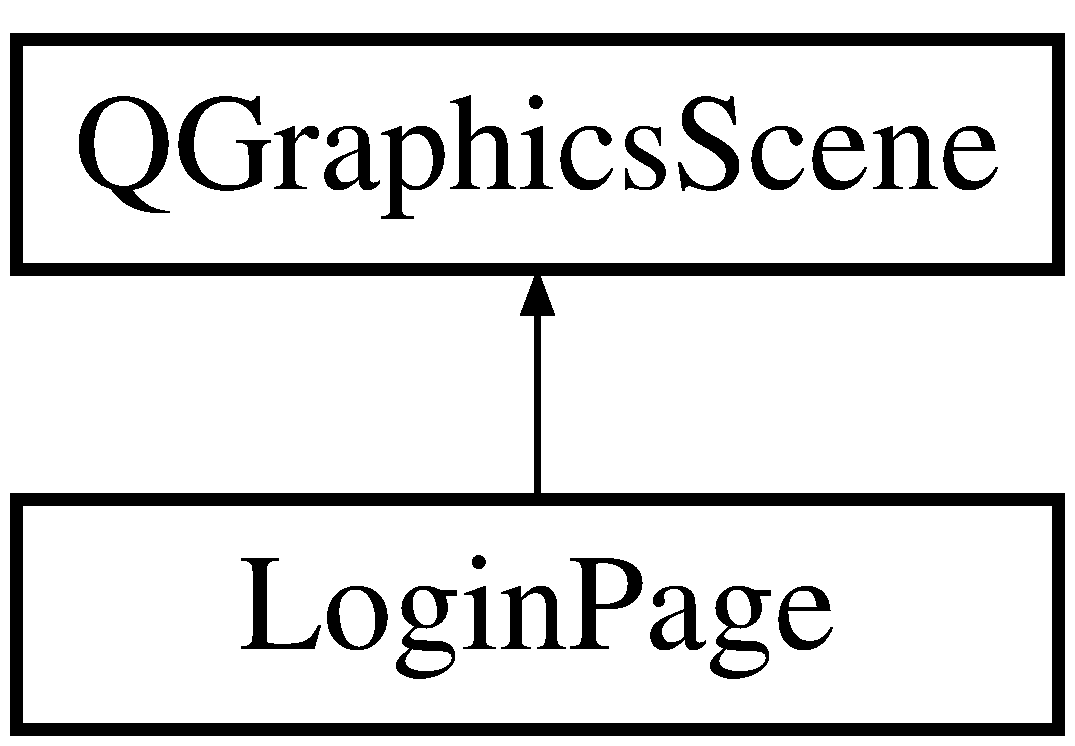
\includegraphics[height=2.000000cm]{classLoginPage}
\end{center}
\end{figure}
\subsection*{Public Slots}
\begin{DoxyCompactItemize}
\item 
void \hyperlink{classLoginPage_a5802453d9b965f17bad2abe14d23ff1c}{login\-User} ()
\end{DoxyCompactItemize}
\subsection*{Public Member Functions}
\begin{DoxyCompactItemize}
\item 
\hypertarget{classLoginPage_ac80d4431cd7779e6ae5f8c3b17fe6c3f}{{\bfseries Login\-Page} (Q\-Widget $\ast$parent=nullptr)}\label{classLoginPage_ac80d4431cd7779e6ae5f8c3b17fe6c3f}

\item 
\hypertarget{classLoginPage_a357fad2a91f6081a2b272ed081dcb014}{void {\bfseries fill\-Scene} ()}\label{classLoginPage_a357fad2a91f6081a2b272ed081dcb014}

\item 
void \hyperlink{classLoginPage_aaa723bfc72a1ba4778e258ba088e0d7a}{fix\-Labels} ()
\end{DoxyCompactItemize}
\subsection*{Public Attributes}
\begin{DoxyCompactItemize}
\item 
\hypertarget{classLoginPage_a1d5dd5716ef5bf6770c48433cccf2974}{\hyperlink{classJson}{Json} {\bfseries json}}\label{classLoginPage_a1d5dd5716ef5bf6770c48433cccf2974}

\item 
\hypertarget{classLoginPage_ae797db11d2d9017001a70515caa38b08}{\hyperlink{classUtil}{Util} {\bfseries util}}\label{classLoginPage_ae797db11d2d9017001a70515caa38b08}

\item 
\hypertarget{classLoginPage_a5f54635b04c4ddd892d719650fd977cc}{\hyperlink{classUser}{User} $\ast$ {\bfseries cur\-User}}\label{classLoginPage_a5f54635b04c4ddd892d719650fd977cc}

\item 
\hypertarget{classLoginPage_a3ec15c43a6e4faf5cda7317167d92721}{Q\-Label $\ast$ {\bfseries login\-Label}}\label{classLoginPage_a3ec15c43a6e4faf5cda7317167d92721}

\item 
\hypertarget{classLoginPage_a4d880e9d90adc87f1e93938de3f8f524}{Q\-Label $\ast$ {\bfseries username\-Label}}\label{classLoginPage_a4d880e9d90adc87f1e93938de3f8f524}

\item 
\hypertarget{classLoginPage_a7d701d4b695ef9c3cf7d2b7116c64427}{Q\-Label $\ast$ {\bfseries password\-Label}}\label{classLoginPage_a7d701d4b695ef9c3cf7d2b7116c64427}

\item 
\hypertarget{classLoginPage_a55a9938b20bfa6e566000bbc10843a54}{Q\-Label $\ast$ {\bfseries no\-Account\-Label}}\label{classLoginPage_a55a9938b20bfa6e566000bbc10843a54}

\item 
\hypertarget{classLoginPage_a4274ac14aa8369d3aaed3b786a760b85}{Q\-Line\-Edit $\ast$ {\bfseries username\-Line\-Edit}}\label{classLoginPage_a4274ac14aa8369d3aaed3b786a760b85}

\item 
\hypertarget{classLoginPage_a7305ba112d1457791d841285a963a04f}{Q\-Line\-Edit $\ast$ {\bfseries password\-Line\-Edit}}\label{classLoginPage_a7305ba112d1457791d841285a963a04f}

\item 
\hypertarget{classLoginPage_acfe1d737483a274558b13dddcfc67f19}{Q\-Push\-Button $\ast$ {\bfseries login\-Button}}\label{classLoginPage_acfe1d737483a274558b13dddcfc67f19}

\item 
\hypertarget{classLoginPage_aef48cad471d0aad88472bf8f703218e2}{Q\-Push\-Button $\ast$ {\bfseries signup\-Button}}\label{classLoginPage_aef48cad471d0aad88472bf8f703218e2}

\item 
\hypertarget{classLoginPage_a1411d81ae64bd5adfcbb4cff160ec4a9}{Q\-Push\-Button $\ast$ {\bfseries home\-Button}}\label{classLoginPage_a1411d81ae64bd5adfcbb4cff160ec4a9}

\end{DoxyCompactItemize}


\subsection{Member Function Documentation}
\hypertarget{classLoginPage_aaa723bfc72a1ba4778e258ba088e0d7a}{\index{Login\-Page@{Login\-Page}!fix\-Labels@{fix\-Labels}}
\index{fix\-Labels@{fix\-Labels}!LoginPage@{Login\-Page}}
\subsubsection[{fix\-Labels}]{\setlength{\rightskip}{0pt plus 5cm}void Login\-Page\-::fix\-Labels (
\begin{DoxyParamCaption}
{}
\end{DoxyParamCaption}
)}}\label{classLoginPage_aaa723bfc72a1ba4778e258ba088e0d7a}
adjusts the design of the labels (color, backround, font, ...) \hypertarget{classLoginPage_a5802453d9b965f17bad2abe14d23ff1c}{\index{Login\-Page@{Login\-Page}!login\-User@{login\-User}}
\index{login\-User@{login\-User}!LoginPage@{Login\-Page}}
\subsubsection[{login\-User}]{\setlength{\rightskip}{0pt plus 5cm}void Login\-Page\-::login\-User (
\begin{DoxyParamCaption}
{}
\end{DoxyParamCaption}
)\hspace{0.3cm}{\ttfamily [slot]}}}\label{classLoginPage_a5802453d9b965f17bad2abe14d23ff1c}
Gets called after a user has attempted to login. using the json.\-cpp utility class\-:
\begin{DoxyItemize}
\item loads the users.\-json file using json.\-get\-Json\-Document()
\item checks if the attempted login was successful using json.\-check\-User(users\-Array,username,password) if successful, the cur\-User instance gets updated to the currently logged in user else, cur\-User becomes N\-U\-L\-L 
\end{DoxyItemize}

The documentation for this class was generated from the following files\-:\begin{DoxyCompactItemize}
\item 
accounts-\/and-\/framework/loginpage.\-h\item 
accounts-\/and-\/framework/loginpage.\-cpp\end{DoxyCompactItemize}

\hypertarget{classMainWindow}{\section{Main\-Window Class Reference}
\label{classMainWindow}\index{Main\-Window@{Main\-Window}}
}
Inheritance diagram for Main\-Window\-:\begin{figure}[H]
\begin{center}
\leavevmode
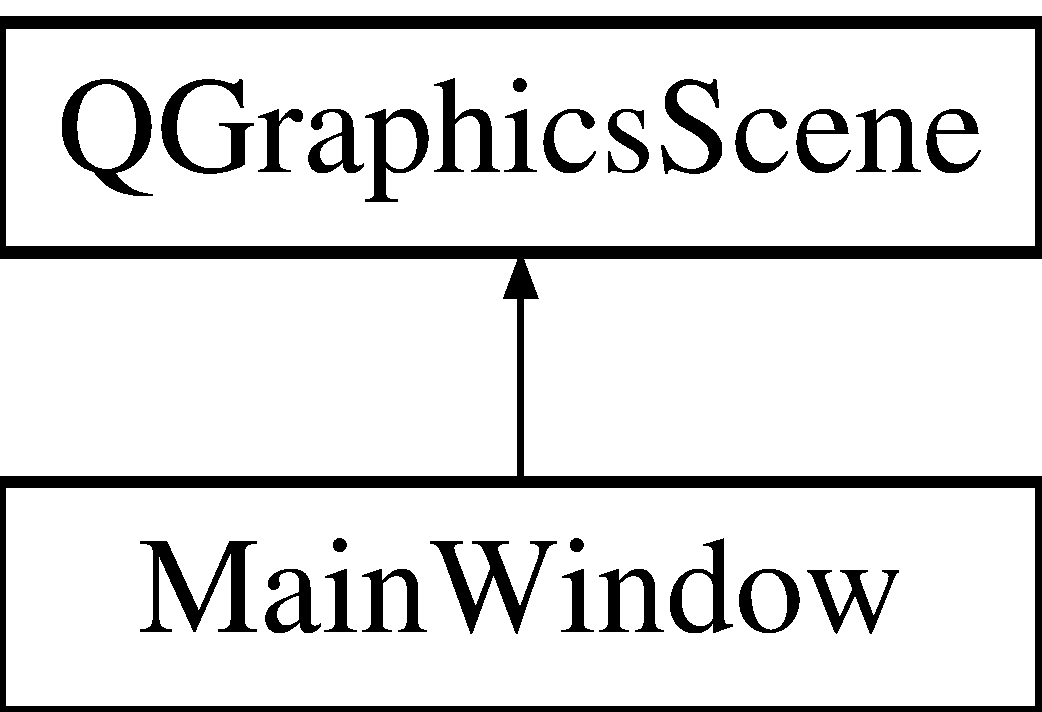
\includegraphics[height=2.000000cm]{classMainWindow}
\end{center}
\end{figure}
\subsection*{Public Member Functions}
\begin{DoxyCompactItemize}
\item 
\hypertarget{classMainWindow_abd384f3538e130501716ded5572c9aef}{void {\bfseries fix\-Labels} ()}\label{classMainWindow_abd384f3538e130501716ded5572c9aef}

\item 
\hypertarget{classMainWindow_ae48d838b0a15efdf4e4ab20edc7ebfcd}{void {\bfseries fill\-Scene} ()}\label{classMainWindow_ae48d838b0a15efdf4e4ab20edc7ebfcd}

\item 
void \hyperlink{classMainWindow_acf4e0d03d562158bfec204334f6de488}{play\-Music} ()
\item 
Q\-String \hyperlink{classMainWindow_a906793bdc362072fc3a5be28fdddfd40}{get\-Joke} ()
\end{DoxyCompactItemize}
\subsection*{Public Attributes}
\begin{DoxyCompactItemize}
\item 
\hypertarget{classMainWindow_a7e5fbafe4ce2c89185cd791f162a4827}{\hyperlink{classJson}{Json} {\bfseries json}}\label{classMainWindow_a7e5fbafe4ce2c89185cd791f162a4827}

\item 
\hypertarget{classMainWindow_a1877ec1952f2fd06f3d3b055b1f08763}{Q\-Label $\ast$ {\bfseries hello\-Label}}\label{classMainWindow_a1877ec1952f2fd06f3d3b055b1f08763}

\item 
\hypertarget{classMainWindow_a78e406c4e1a86c9ecacaf1de4b1c3196}{Q\-Label $\ast$ {\bfseries joke\-Label}}\label{classMainWindow_a78e406c4e1a86c9ecacaf1de4b1c3196}

\item 
\hypertarget{classMainWindow_a6922a5979d220eec99dacdebe8d4cfae}{Q\-Label $\ast$ {\bfseries joke}}\label{classMainWindow_a6922a5979d220eec99dacdebe8d4cfae}

\item 
\hypertarget{classMainWindow_aa0b3757bd2a0b71a40393fff4a07c64b}{Q\-Push\-Button $\ast$ {\bfseries login\-Button}}\label{classMainWindow_aa0b3757bd2a0b71a40393fff4a07c64b}

\item 
\hypertarget{classMainWindow_a71e4a8d71f472f15bee72e43650f2b78}{Q\-Push\-Button $\ast$ {\bfseries signup\-Button}}\label{classMainWindow_a71e4a8d71f472f15bee72e43650f2b78}

\item 
\hypertarget{classMainWindow_afd28c3e2ac187140050cf0ea82d6b85d}{Q\-Push\-Button $\ast$ {\bfseries guest\-Button}}\label{classMainWindow_afd28c3e2ac187140050cf0ea82d6b85d}

\end{DoxyCompactItemize}


\subsection{Member Function Documentation}
\hypertarget{classMainWindow_a906793bdc362072fc3a5be28fdddfd40}{\index{Main\-Window@{Main\-Window}!get\-Joke@{get\-Joke}}
\index{get\-Joke@{get\-Joke}!MainWindow@{Main\-Window}}
\subsubsection[{get\-Joke}]{\setlength{\rightskip}{0pt plus 5cm}Q\-String Main\-Window\-::get\-Joke (
\begin{DoxyParamCaption}
{}
\end{DoxyParamCaption}
)}}\label{classMainWindow_a906793bdc362072fc3a5be28fdddfd40}
loads the jokes.\-json document selects a random joke from it

\begin{DoxyReturn}{Returns}
Q\-String as a Joke. 
\end{DoxyReturn}
\hypertarget{classMainWindow_acf4e0d03d562158bfec204334f6de488}{\index{Main\-Window@{Main\-Window}!play\-Music@{play\-Music}}
\index{play\-Music@{play\-Music}!MainWindow@{Main\-Window}}
\subsubsection[{play\-Music}]{\setlength{\rightskip}{0pt plus 5cm}void Main\-Window\-::play\-Music (
\begin{DoxyParamCaption}
{}
\end{DoxyParamCaption}
)}}\label{classMainWindow_acf4e0d03d562158bfec204334f6de488}
Set the Background music. 

The documentation for this class was generated from the following files\-:\begin{DoxyCompactItemize}
\item 
accounts-\/and-\/framework/mainwindow.\-h\item 
accounts-\/and-\/framework/mainwindow.\-cpp\end{DoxyCompactItemize}

\hypertarget{classPoint}{\section{Point Class Reference}
\label{classPoint}\index{Point@{Point}}
}
\subsection*{Public Member Functions}
\begin{DoxyCompactItemize}
\item 
\hypertarget{classPoint_adcee15014d4b11143ecfc9afffe6a338}{bool {\bfseries operator!=} (\hyperlink{classPoint}{Point} point)}\label{classPoint_adcee15014d4b11143ecfc9afffe6a338}

\item 
\hypertarget{classPoint_ab5e7dc8e63dae82bc88456125b957482}{bool {\bfseries operator==} (\hyperlink{classPoint}{Point} point)}\label{classPoint_ab5e7dc8e63dae82bc88456125b957482}

\item 
\hypertarget{classPoint_a001c4958c310b248f5c26037aea38a9c}{{\bfseries Point} (int x, int y)}\label{classPoint_a001c4958c310b248f5c26037aea38a9c}

\end{DoxyCompactItemize}
\subsection*{Public Attributes}
\begin{DoxyCompactItemize}
\item 
\hypertarget{classPoint_a8c779e11e694b20e0946105a9f5de842}{int {\bfseries x}}\label{classPoint_a8c779e11e694b20e0946105a9f5de842}

\item 
\hypertarget{classPoint_a2e1b5fb2b2a83571f5c0bc0f66a73cf7}{int {\bfseries y}}\label{classPoint_a2e1b5fb2b2a83571f5c0bc0f66a73cf7}

\end{DoxyCompactItemize}


The documentation for this class was generated from the following files\-:\begin{DoxyCompactItemize}
\item 
game-\/2-\/reversi/point.\-h\item 
game-\/2-\/reversi/point.\-cpp\end{DoxyCompactItemize}

\hypertarget{classRollingBg}{\section{Rolling\-Bg Class Reference}
\label{classRollingBg}\index{Rolling\-Bg@{Rolling\-Bg}}
}
Inheritance diagram for Rolling\-Bg\-:\begin{figure}[H]
\begin{center}
\leavevmode
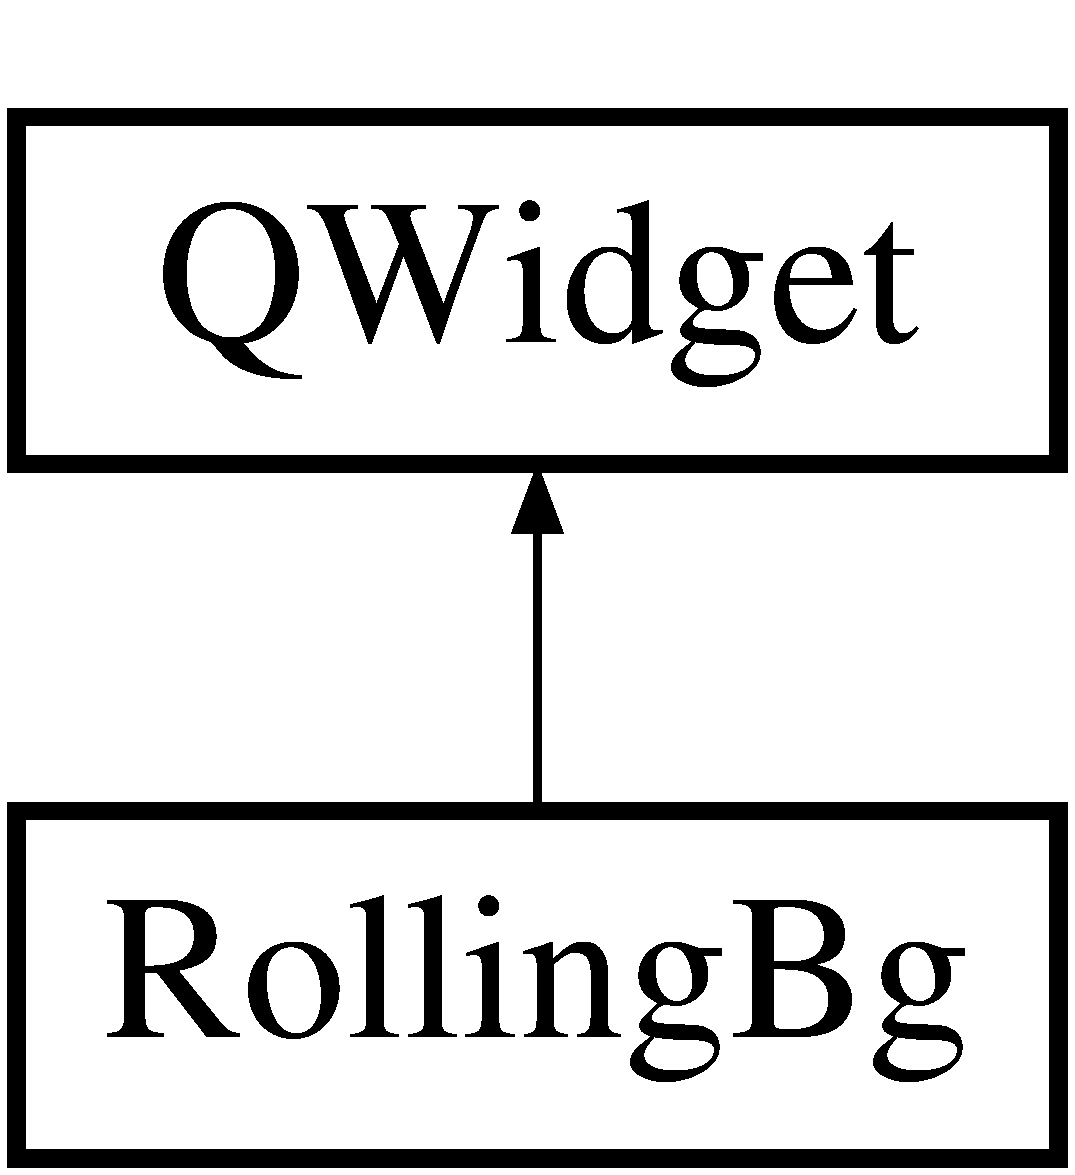
\includegraphics[height=2.000000cm]{classRollingBg}
\end{center}
\end{figure}
\subsection*{Public Member Functions}
\begin{DoxyCompactItemize}
\item 
\hypertarget{classRollingBg_ab26828e307d50620a0a6f03fcbb2e591}{{\bfseries Rolling\-Bg} (Q\-Widget $\ast$parent=nullptr)}\label{classRollingBg_ab26828e307d50620a0a6f03fcbb2e591}

\end{DoxyCompactItemize}
\subsection*{Public Attributes}
\begin{DoxyCompactItemize}
\item 
\hypertarget{classRollingBg_a254dd1f63ac2d916290f477d34099841}{Q\-Timer $\ast$ {\bfseries timer}}\label{classRollingBg_a254dd1f63ac2d916290f477d34099841}

\item 
\hypertarget{classRollingBg_a40c01dec8cb9774ddfd80e3522c1cf82}{int {\bfseries timer\-Speed} = 50}\label{classRollingBg_a40c01dec8cb9774ddfd80e3522c1cf82}

\end{DoxyCompactItemize}
\subsection*{Protected Member Functions}
\begin{DoxyCompactItemize}
\item 
void \hyperlink{classRollingBg_adaae6dcc6b9b655bc76bfe06802482d5}{paint\-Event} (Q\-Paint\-Event $\ast$event) override
\end{DoxyCompactItemize}


\subsection{Member Function Documentation}
\hypertarget{classRollingBg_adaae6dcc6b9b655bc76bfe06802482d5}{\index{Rolling\-Bg@{Rolling\-Bg}!paint\-Event@{paint\-Event}}
\index{paint\-Event@{paint\-Event}!RollingBg@{Rolling\-Bg}}
\subsubsection[{paint\-Event}]{\setlength{\rightskip}{0pt plus 5cm}void Rolling\-Bg\-::paint\-Event (
\begin{DoxyParamCaption}
\item[{Q\-Paint\-Event $\ast$}]{event}
\end{DoxyParamCaption}
)\hspace{0.3cm}{\ttfamily [override]}, {\ttfamily [protected]}}}\label{classRollingBg_adaae6dcc6b9b655bc76bfe06802482d5}
A function to create a Q\-Painter and draw on it 

The documentation for this class was generated from the following files\-:\begin{DoxyCompactItemize}
\item 
game1-\/kill-\/covid-\/19/rollingbg.\-h\item 
game1-\/kill-\/covid-\/19/rollingbg.\-cpp\end{DoxyCompactItemize}

\hypertarget{classSignupPage}{\section{Signup\-Page Class Reference}
\label{classSignupPage}\index{Signup\-Page@{Signup\-Page}}
}
Inheritance diagram for Signup\-Page\-:\begin{figure}[H]
\begin{center}
\leavevmode
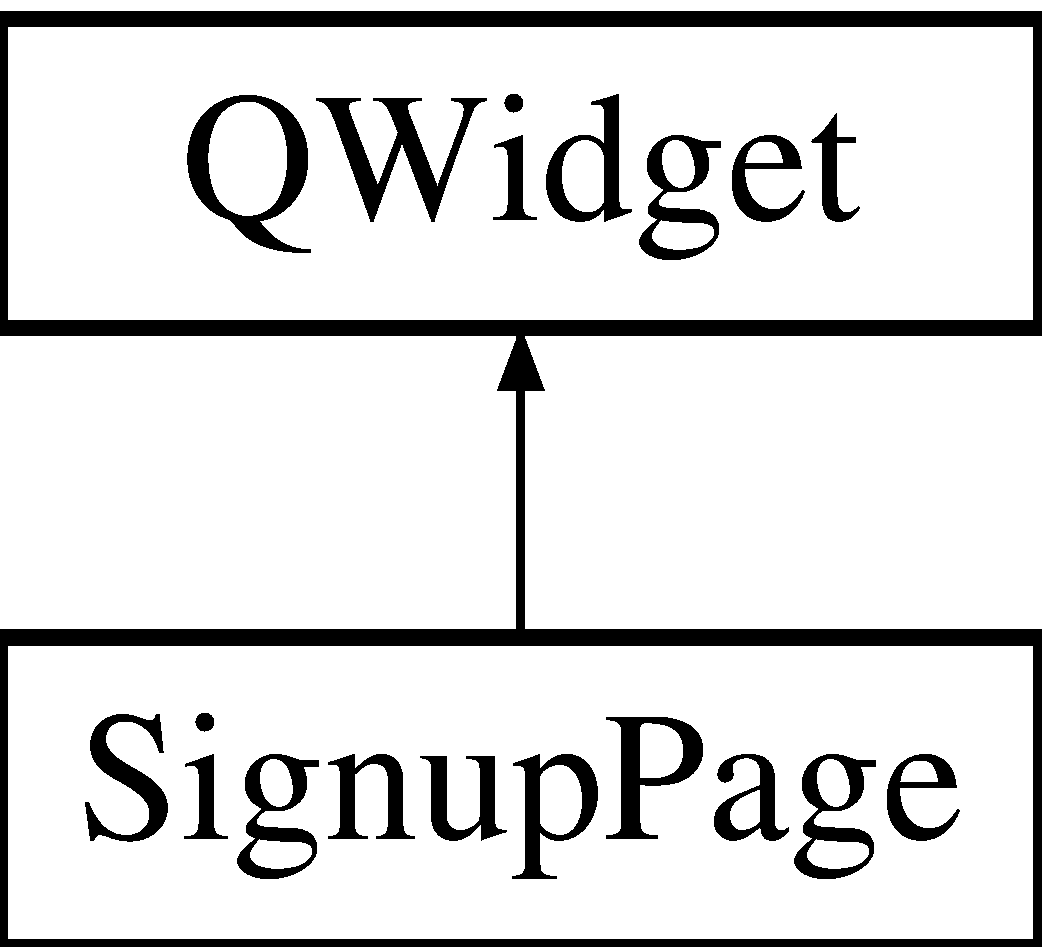
\includegraphics[height=2.000000cm]{classSignupPage}
\end{center}
\end{figure}
\subsection*{Public Slots}
\begin{DoxyCompactItemize}
\item 
void \hyperlink{classSignupPage_ab42434ae99ddc49856abdf513ae80884}{set\-User} ()
\item 
void \hyperlink{classSignupPage_abdb7ff1100d852d074c9724cf695ab06}{select\-Image} ()
\end{DoxyCompactItemize}
\subsection*{Public Member Functions}
\begin{DoxyCompactItemize}
\item 
\hypertarget{classSignupPage_af41bce1fd7c7e7f6b78e7dd0e790f1c5}{{\bfseries Signup\-Page} (Q\-Widget $\ast$parent=nullptr)}\label{classSignupPage_af41bce1fd7c7e7f6b78e7dd0e790f1c5}

\item 
\hyperlink{classUser}{User} $\ast$ \hyperlink{classSignupPage_ac6f433285ca77bcfa6bae1d3b37cd5b5}{create\-User} ()
\item 
void \hyperlink{classSignupPage_aef2b54e11fa46f9c887e696a7eb9d786}{clean\-Page} ()
\end{DoxyCompactItemize}
\subsection*{Public Attributes}
\begin{DoxyCompactItemize}
\item 
\hypertarget{classSignupPage_aeae60650678de2e566170694a117cce0}{\hyperlink{classUser}{User} $\ast$ {\bfseries cur\-User} = N\-U\-L\-L}\label{classSignupPage_aeae60650678de2e566170694a117cce0}

\item 
\hypertarget{classSignupPage_af31808c1416a401aa65942abd91c134d}{\hyperlink{classJson}{Json} {\bfseries json}}\label{classSignupPage_af31808c1416a401aa65942abd91c134d}

\item 
\hypertarget{classSignupPage_a40679fa25d422bc6f7616c8bb332b51d}{\hyperlink{classUtil}{Util} {\bfseries util}}\label{classSignupPage_a40679fa25d422bc6f7616c8bb332b51d}

\item 
\hypertarget{classSignupPage_a669d0f940516c7c3be821b13e240a8ba}{Q\-Label $\ast$ {\bfseries Header}}\label{classSignupPage_a669d0f940516c7c3be821b13e240a8ba}

\item 
\hypertarget{classSignupPage_a2d334ba2d8cc80d5cd841045834db0c7}{Q\-Label $\ast$ {\bfseries Sign\-In\-Label}}\label{classSignupPage_a2d334ba2d8cc80d5cd841045834db0c7}

\item 
\hypertarget{classSignupPage_ad32e82ef305d5c52ee094a883d9922f8}{Q\-Line\-Edit $\ast$ {\bfseries First\-Name\-Edit}}\label{classSignupPage_ad32e82ef305d5c52ee094a883d9922f8}

\item 
\hypertarget{classSignupPage_aa76f41a9f446ec85369f1173e212a432}{Q\-Line\-Edit $\ast$ {\bfseries Second\-Name\-Edit}}\label{classSignupPage_aa76f41a9f446ec85369f1173e212a432}

\item 
\hypertarget{classSignupPage_a603f414386b5dee21a7f240c2a7c63ce}{Q\-Line\-Edit $\ast$ {\bfseries Username\-Edit}}\label{classSignupPage_a603f414386b5dee21a7f240c2a7c63ce}

\item 
\hypertarget{classSignupPage_af8d1413ac72df4295c7d539b675bf998}{Q\-Line\-Edit $\ast$ {\bfseries Password\-Edit}}\label{classSignupPage_af8d1413ac72df4295c7d539b675bf998}

\item 
\hypertarget{classSignupPage_acaa25d70cad45913c45ee98c67c97d6e}{Q\-Line\-Edit $\ast$ {\bfseries Confirm\-Password\-Edit}}\label{classSignupPage_acaa25d70cad45913c45ee98c67c97d6e}

\item 
\hypertarget{classSignupPage_a40bf3b798d78448ff4517ee01f9dd50c}{Q\-Combo\-Box $\ast$ {\bfseries Gender\-Box}}\label{classSignupPage_a40bf3b798d78448ff4517ee01f9dd50c}

\item 
\hypertarget{classSignupPage_ab8d5ae4f47f250ee6c06281b2dd84bb3}{Q\-Spin\-Box $\ast$ {\bfseries Age\-Box}}\label{classSignupPage_ab8d5ae4f47f250ee6c06281b2dd84bb3}

\item 
\hypertarget{classSignupPage_aa8e984ee0df799e8bf653ba2ef09e173}{Q\-Spin\-Box $\ast$ {\bfseries Day\-Box}}\label{classSignupPage_aa8e984ee0df799e8bf653ba2ef09e173}

\item 
\hypertarget{classSignupPage_a5101c02eba181948b92da7c228160c0f}{Q\-Spin\-Box $\ast$ {\bfseries Month\-Box}}\label{classSignupPage_a5101c02eba181948b92da7c228160c0f}

\item 
\hypertarget{classSignupPage_acc094cbb7857d78cbd09def2bdb9e774}{Q\-Spin\-Box $\ast$ {\bfseries Year\-Box}}\label{classSignupPage_acc094cbb7857d78cbd09def2bdb9e774}

\item 
\hypertarget{classSignupPage_ac5fda5032a203021b57332163040d0d6}{Q\-Push\-Button $\ast$ {\bfseries Sign\-Up\-Button}}\label{classSignupPage_ac5fda5032a203021b57332163040d0d6}

\item 
\hypertarget{classSignupPage_a9fea25d5db1e6b70cbb8896e71fd592c}{Q\-Push\-Button $\ast$ {\bfseries Sign\-In\-Button}}\label{classSignupPage_a9fea25d5db1e6b70cbb8896e71fd592c}

\item 
\hypertarget{classSignupPage_a42c8bc45059bad0cdcb57859df207fa8}{Q\-Push\-Button $\ast$ {\bfseries Select\-Image}}\label{classSignupPage_a42c8bc45059bad0cdcb57859df207fa8}

\item 
\hypertarget{classSignupPage_a60dd16dbed5dbebf92474c8e7f948c24}{Q\-V\-Box\-Layout $\ast$ {\bfseries Box\-Layout}}\label{classSignupPage_a60dd16dbed5dbebf92474c8e7f948c24}

\item 
\hypertarget{classSignupPage_ac93a28fff319901d4a55060329676bc9}{Q\-Form\-Layout $\ast$ {\bfseries Form\-Layout}}\label{classSignupPage_ac93a28fff319901d4a55060329676bc9}

\item 
\hypertarget{classSignupPage_a56380dc42c5757d57b63d6d7a91cdcf9}{Q\-H\-Box\-Layout $\ast$ {\bfseries Date\-Layout}}\label{classSignupPage_a56380dc42c5757d57b63d6d7a91cdcf9}

\item 
\hypertarget{classSignupPage_afd9ce0fc5b06863c24a908b9af522130}{Q\-H\-Box\-Layout $\ast$ {\bfseries Sign\-In\-Layout}}\label{classSignupPage_afd9ce0fc5b06863c24a908b9af522130}

\item 
\hypertarget{classSignupPage_a41cace8c3f21b6314544dfae8fe0b0cf}{Q\-Group\-Box $\ast$ {\bfseries Group\-Box}}\label{classSignupPage_a41cace8c3f21b6314544dfae8fe0b0cf}

\item 
\hypertarget{classSignupPage_a28a68ef95b6d206d616df6e7c25913f9}{Q\-String {\bfseries file\-\_\-name}}\label{classSignupPage_a28a68ef95b6d206d616df6e7c25913f9}

\end{DoxyCompactItemize}


\subsection{Member Function Documentation}
\hypertarget{classSignupPage_aef2b54e11fa46f9c887e696a7eb9d786}{\index{Signup\-Page@{Signup\-Page}!clean\-Page@{clean\-Page}}
\index{clean\-Page@{clean\-Page}!SignupPage@{Signup\-Page}}
\subsubsection[{clean\-Page}]{\setlength{\rightskip}{0pt plus 5cm}void Signup\-Page\-::clean\-Page (
\begin{DoxyParamCaption}
{}
\end{DoxyParamCaption}
)}}\label{classSignupPage_aef2b54e11fa46f9c887e696a7eb9d786}

\begin{DoxyItemize}
\item this methods resets all the widgets that took user input
\item Gets called whenever a user wants to signup 
\end{DoxyItemize}\hypertarget{classSignupPage_ac6f433285ca77bcfa6bae1d3b37cd5b5}{\index{Signup\-Page@{Signup\-Page}!create\-User@{create\-User}}
\index{create\-User@{create\-User}!SignupPage@{Signup\-Page}}
\subsubsection[{create\-User}]{\setlength{\rightskip}{0pt plus 5cm}{\bf User} $\ast$ Signup\-Page\-::create\-User (
\begin{DoxyParamCaption}
{}
\end{DoxyParamCaption}
)}}\label{classSignupPage_ac6f433285ca77bcfa6bae1d3b37cd5b5}
called from the \hyperlink{classSignupPage_ab42434ae99ddc49856abdf513ae80884}{set\-User()} S\-L\-O\-T Reads the input from the widgets and attemps to create a new user

\begin{DoxyReturn}{Returns}
if successful, returns the new user (not yet added to users.\-json) else, returns N\-U\-L\-L 
\end{DoxyReturn}
\hypertarget{classSignupPage_abdb7ff1100d852d074c9724cf695ab06}{\index{Signup\-Page@{Signup\-Page}!select\-Image@{select\-Image}}
\index{select\-Image@{select\-Image}!SignupPage@{Signup\-Page}}
\subsubsection[{select\-Image}]{\setlength{\rightskip}{0pt plus 5cm}void Signup\-Page\-::select\-Image (
\begin{DoxyParamCaption}
{}
\end{DoxyParamCaption}
)\hspace{0.3cm}{\ttfamily [slot]}}}\label{classSignupPage_abdb7ff1100d852d074c9724cf695ab06}
Takes profile picture file path from user updates the corresponding class member \hypertarget{classSignupPage_ab42434ae99ddc49856abdf513ae80884}{\index{Signup\-Page@{Signup\-Page}!set\-User@{set\-User}}
\index{set\-User@{set\-User}!SignupPage@{Signup\-Page}}
\subsubsection[{set\-User}]{\setlength{\rightskip}{0pt plus 5cm}void Signup\-Page\-::set\-User (
\begin{DoxyParamCaption}
{}
\end{DoxyParamCaption}
)\hspace{0.3cm}{\ttfamily [slot]}}}\label{classSignupPage_ab42434ae99ddc49856abdf513ae80884}
Called whenever the signup button is pressed calls \hyperlink{classSignupPage_ac6f433285ca77bcfa6bae1d3b37cd5b5}{create\-User()} in order to check all necessary conditions before adding a new user to the users.\-json file if \hyperlink{classSignupPage_ac6f433285ca77bcfa6bae1d3b37cd5b5}{create\-User()} returned a user, \hyperlink{classSignupPage_ab42434ae99ddc49856abdf513ae80884}{set\-User()} appends it to users.\-json 

The documentation for this class was generated from the following files\-:\begin{DoxyCompactItemize}
\item 
accounts-\/and-\/framework/signuppage.\-h\item 
accounts-\/and-\/framework/signuppage.\-cpp\end{DoxyCompactItemize}

\hypertarget{classStrategy}{\section{Strategy Class Reference}
\label{classStrategy}\index{Strategy@{Strategy}}
}
\subsection*{Public Member Functions}
\begin{DoxyCompactItemize}
\item 
\hypertarget{classStrategy_a21c7057471c611cae5e7570ec8ead85b}{{\bfseries Strategy} (int player)}\label{classStrategy_a21c7057471c611cae5e7570ec8ead85b}

\item 
void \hyperlink{classStrategy_a59ea7b1415dac94fd8c919d2255bf6c0}{play} (\hyperlink{classBoard}{Board} $\ast$board)
\end{DoxyCompactItemize}


\subsection{Member Function Documentation}
\hypertarget{classStrategy_a59ea7b1415dac94fd8c919d2255bf6c0}{\index{Strategy@{Strategy}!play@{play}}
\index{play@{play}!Strategy@{Strategy}}
\subsubsection[{play}]{\setlength{\rightskip}{0pt plus 5cm}void Strategy\-::play (
\begin{DoxyParamCaption}
\item[{{\bf Board} $\ast$}]{board}
\end{DoxyParamCaption}
)}}\label{classStrategy_a59ea7b1415dac94fd8c919d2255bf6c0}
A funciton used by the A\-I to play its strategy 

The documentation for this class was generated from the following files\-:\begin{DoxyCompactItemize}
\item 
game-\/2-\/reversi/strategy.\-h\item 
game-\/2-\/reversi/strategy.\-cpp\end{DoxyCompactItemize}

\hypertarget{classSyringe}{\section{Syringe Class Reference}
\label{classSyringe}\index{Syringe@{Syringe}}
}
Inheritance diagram for Syringe\-:\begin{figure}[H]
\begin{center}
\leavevmode
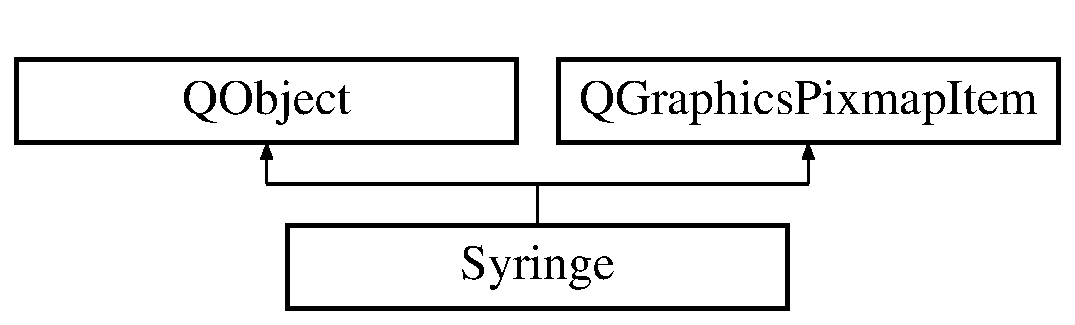
\includegraphics[height=2.000000cm]{classSyringe}
\end{center}
\end{figure}
\subsection*{Public Member Functions}
\begin{DoxyCompactItemize}
\item 
\hypertarget{classSyringe_a23cd14bbda9d49bf21a66f6606a7baab}{{\bfseries Syringe} (Q\-Object $\ast$parent=nullptr)}\label{classSyringe_a23cd14bbda9d49bf21a66f6606a7baab}

\end{DoxyCompactItemize}
\subsection*{Public Attributes}
\begin{DoxyCompactItemize}
\item 
\hypertarget{classSyringe_a4408fc94be7fab5785d86afde994d7d0}{Q\-String {\bfseries syringe\-Pic\-Path} = \char`\"{}\-:/game1images/syringe.\-png\char`\"{}}\label{classSyringe_a4408fc94be7fab5785d86afde994d7d0}

\end{DoxyCompactItemize}


The documentation for this class was generated from the following files\-:\begin{DoxyCompactItemize}
\item 
game1-\/kill-\/covid-\/19/syringe.\-h\item 
game1-\/kill-\/covid-\/19/syringe.\-cpp\end{DoxyCompactItemize}

\hypertarget{classUser}{\section{User Class Reference}
\label{classUser}\index{User@{User}}
}
Inheritance diagram for User\-:\begin{figure}[H]
\begin{center}
\leavevmode
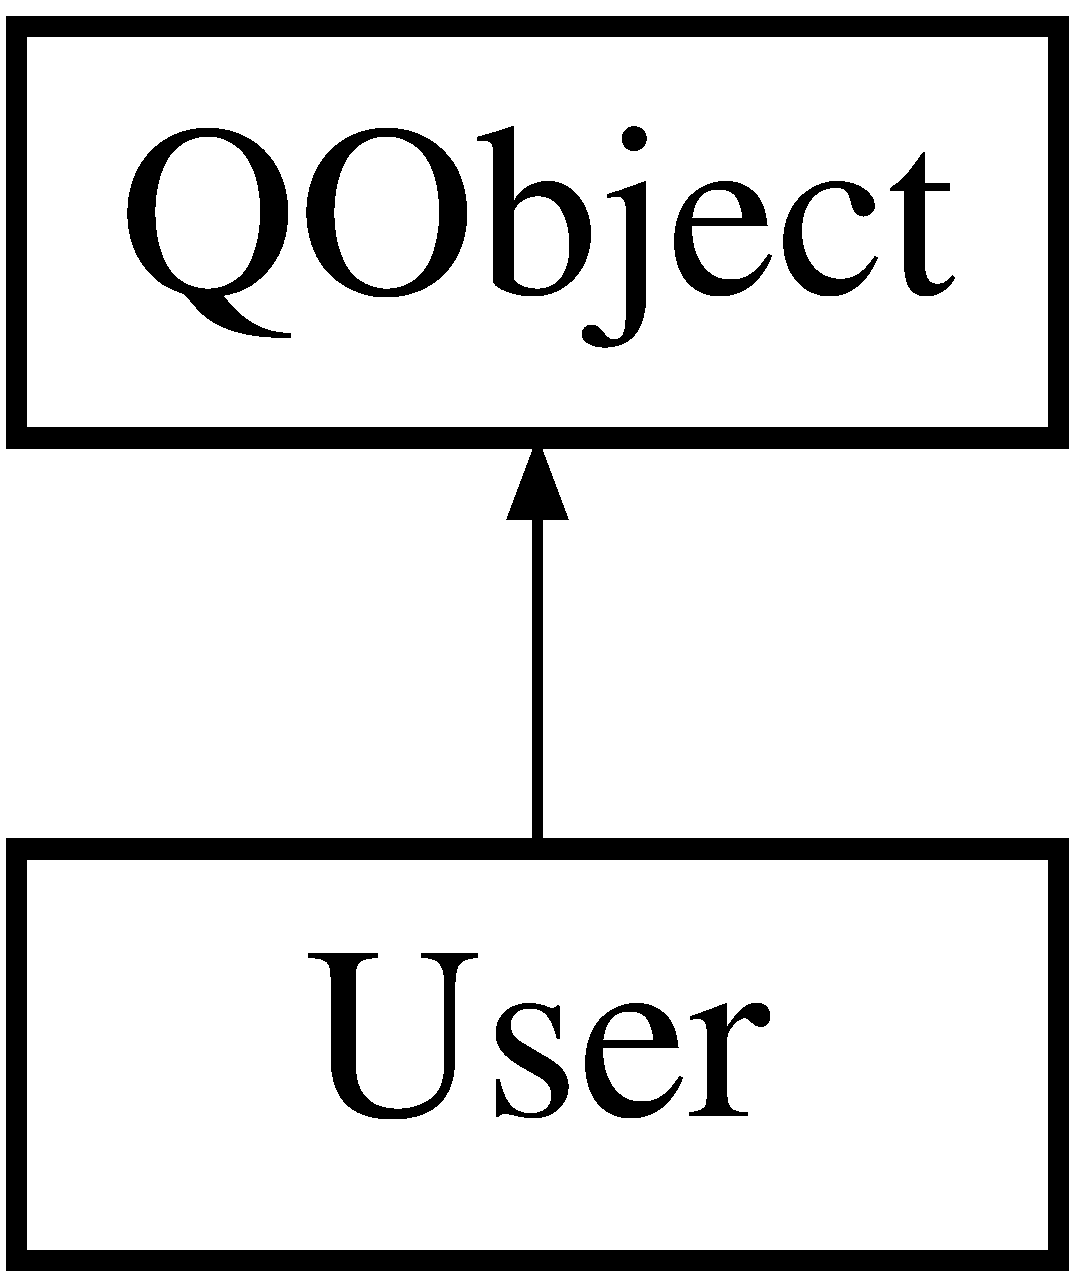
\includegraphics[height=2.000000cm]{classUser}
\end{center}
\end{figure}
\subsection*{Public Member Functions}
\begin{DoxyCompactItemize}
\item 
\hypertarget{classUser_ae90821c4c8cc9a5a370f0ad6157adcc1}{{\bfseries User} (Q\-Object $\ast$parent=nullptr)}\label{classUser_ae90821c4c8cc9a5a370f0ad6157adcc1}

\item 
\hyperlink{classUser_a46c2dbdb8006a8752de309a81694a15b}{User} (Q\-Json\-Object user\-Json)
\item 
\hypertarget{classUser_ab12a51628183409d7ca7254fc67d7fbf}{void {\bfseries read} (const Q\-Json\-Object \&json)}\label{classUser_ab12a51628183409d7ca7254fc67d7fbf}

\item 
\hypertarget{classUser_a5a31456667d33c587e92aa0978612cac}{void {\bfseries write} (Q\-Json\-Object \&json) const }\label{classUser_a5a31456667d33c587e92aa0978612cac}

\item 
bool \hyperlink{classUser_a9e1fe4ac5c94a98f82ca09fa0982e029}{is\-Unique} ()
\item 
bool \hyperlink{classUser_a7fff50444765760051f4ae6fb3d58e16}{is\-Valid} ()
\item 
Q\-Json\-Object \hyperlink{classUser_aad36c436bfe69348e114fd922f9597ba}{to\-Json\-Object} ()
\item 
Q\-Json\-Array \hyperlink{classUser_a66d5ee177223841933f3907bf9a8362b}{get\-Scores\-As\-Json} (Q\-Vector$<$ int $>$ \&scores)
\end{DoxyCompactItemize}
\subsection*{Public Attributes}
\begin{DoxyCompactItemize}
\item 
\hypertarget{classUser_ab0ffba62281ba773094d3f7e9cb1b861}{\hyperlink{classJson}{Json} {\bfseries json}}\label{classUser_ab0ffba62281ba773094d3f7e9cb1b861}

\item 
\hypertarget{classUser_aed78465b35175ff33ab3ca3ca1ebe450}{Q\-String {\bfseries first\-Name}}\label{classUser_aed78465b35175ff33ab3ca3ca1ebe450}

\item 
\hypertarget{classUser_a3a225093bbb405dab285e74e24cef7c5}{Q\-String {\bfseries last\-Name}}\label{classUser_a3a225093bbb405dab285e74e24cef7c5}

\item 
\hypertarget{classUser_ae7cf3e04e6aba46f20af4c6802630074}{Q\-String {\bfseries gender}}\label{classUser_ae7cf3e04e6aba46f20af4c6802630074}

\item 
\hypertarget{classUser_ae4202de2b7974e92a55b913d20b03833}{Q\-String {\bfseries username}}\label{classUser_ae4202de2b7974e92a55b913d20b03833}

\item 
\hypertarget{classUser_acdd1a26c7a5fa4d241af640e3ff00c37}{Q\-String {\bfseries date\-Of\-Birth}}\label{classUser_acdd1a26c7a5fa4d241af640e3ff00c37}

\item 
\hypertarget{classUser_a1a118876605a4a27e37b4a9ececded5a}{Q\-Json\-Value {\bfseries picture}}\label{classUser_a1a118876605a4a27e37b4a9ececded5a}

\item 
\hypertarget{classUser_a0c6d93f685111e10b940e7e96dbac6a6}{int {\bfseries hashedpassword}}\label{classUser_a0c6d93f685111e10b940e7e96dbac6a6}

\item 
\hypertarget{classUser_aa5829689588d1f982e1a69b73bd68655}{int {\bfseries age}}\label{classUser_aa5829689588d1f982e1a69b73bd68655}

\item 
\hypertarget{classUser_aa2de22213dd79246b98e22e6d92def88}{int {\bfseries game1\-\_\-highest} = 0}\label{classUser_aa2de22213dd79246b98e22e6d92def88}

\item 
\hypertarget{classUser_a17a375d0735e08067c33b0e5bd39e55c}{int {\bfseries game2\-\_\-highest} = 0}\label{classUser_a17a375d0735e08067c33b0e5bd39e55c}

\item 
\hypertarget{classUser_a6337f4e2388a6eb3322940662db8ff45}{Q\-Vector$<$ int $>$ {\bfseries game1\-\_\-scores} = \{0,0,0,0,0\}}\label{classUser_a6337f4e2388a6eb3322940662db8ff45}

\item 
\hypertarget{classUser_a1b527baf64748d4a8d94c88c0e1632af}{Q\-Vector$<$ int $>$ {\bfseries game2\-\_\-scores} = \{0,0,0,0,0\}}\label{classUser_a1b527baf64748d4a8d94c88c0e1632af}

\end{DoxyCompactItemize}


\subsection{Constructor \& Destructor Documentation}
\hypertarget{classUser_a46c2dbdb8006a8752de309a81694a15b}{\index{User@{User}!User@{User}}
\index{User@{User}!User@{User}}
\subsubsection[{User}]{\setlength{\rightskip}{0pt plus 5cm}User\-::\-User (
\begin{DoxyParamCaption}
\item[{Q\-Json\-Object}]{result}
\end{DoxyParamCaption}
)\hspace{0.3cm}{\ttfamily [explicit]}}}\label{classUser_a46c2dbdb8006a8752de309a81694a15b}
Gets the \hyperlink{classUser}{User} from a Q\-Json\-Object

\begin{DoxyReturn}{Returns}
a user from the users.\-json 
\end{DoxyReturn}


\subsection{Member Function Documentation}
\hypertarget{classUser_a66d5ee177223841933f3907bf9a8362b}{\index{User@{User}!get\-Scores\-As\-Json@{get\-Scores\-As\-Json}}
\index{get\-Scores\-As\-Json@{get\-Scores\-As\-Json}!User@{User}}
\subsubsection[{get\-Scores\-As\-Json}]{\setlength{\rightskip}{0pt plus 5cm}Q\-Json\-Array User\-::get\-Scores\-As\-Json (
\begin{DoxyParamCaption}
\item[{Q\-Vector$<$ int $>$ \&}]{scores}
\end{DoxyParamCaption}
)}}\label{classUser_a66d5ee177223841933f3907bf9a8362b}
Transforms a vector of scores to Q\-Json\-Array \begin{DoxyReturn}{Returns}
Q\-Json\-Array of scores 
\end{DoxyReturn}
\hypertarget{classUser_a9e1fe4ac5c94a98f82ca09fa0982e029}{\index{User@{User}!is\-Unique@{is\-Unique}}
\index{is\-Unique@{is\-Unique}!User@{User}}
\subsubsection[{is\-Unique}]{\setlength{\rightskip}{0pt plus 5cm}bool User\-::is\-Unique (
\begin{DoxyParamCaption}
{}
\end{DoxyParamCaption}
)}}\label{classUser_a9e1fe4ac5c94a98f82ca09fa0982e029}
Checks whether a \hyperlink{classUser}{User} is unique or not \begin{DoxyReturn}{Returns}
True if unique, False otherwise. 
\end{DoxyReturn}
\hypertarget{classUser_a7fff50444765760051f4ae6fb3d58e16}{\index{User@{User}!is\-Valid@{is\-Valid}}
\index{is\-Valid@{is\-Valid}!User@{User}}
\subsubsection[{is\-Valid}]{\setlength{\rightskip}{0pt plus 5cm}bool User\-::is\-Valid (
\begin{DoxyParamCaption}
{}
\end{DoxyParamCaption}
)}}\label{classUser_a7fff50444765760051f4ae6fb3d58e16}
Checks whether \hyperlink{classUser}{User}'s input is valid \begin{DoxyReturn}{Returns}
true if valid, false otherwise. 
\end{DoxyReturn}
\hypertarget{classUser_aad36c436bfe69348e114fd922f9597ba}{\index{User@{User}!to\-Json\-Object@{to\-Json\-Object}}
\index{to\-Json\-Object@{to\-Json\-Object}!User@{User}}
\subsubsection[{to\-Json\-Object}]{\setlength{\rightskip}{0pt plus 5cm}Q\-Json\-Object User\-::to\-Json\-Object (
\begin{DoxyParamCaption}
{}
\end{DoxyParamCaption}
)}}\label{classUser_aad36c436bfe69348e114fd922f9597ba}
Transforms a \hyperlink{classUser}{User} to a Q\-Json\-Object \begin{DoxyReturn}{Returns}
Corresponding Q\-Json\-Object 
\end{DoxyReturn}


The documentation for this class was generated from the following files\-:\begin{DoxyCompactItemize}
\item 
accounts-\/and-\/framework/user.\-h\item 
accounts-\/and-\/framework/user.\-cpp\end{DoxyCompactItemize}

\hypertarget{classUtil}{\section{Util Class Reference}
\label{classUtil}\index{Util@{Util}}
}
Inheritance diagram for Util\-:\begin{figure}[H]
\begin{center}
\leavevmode
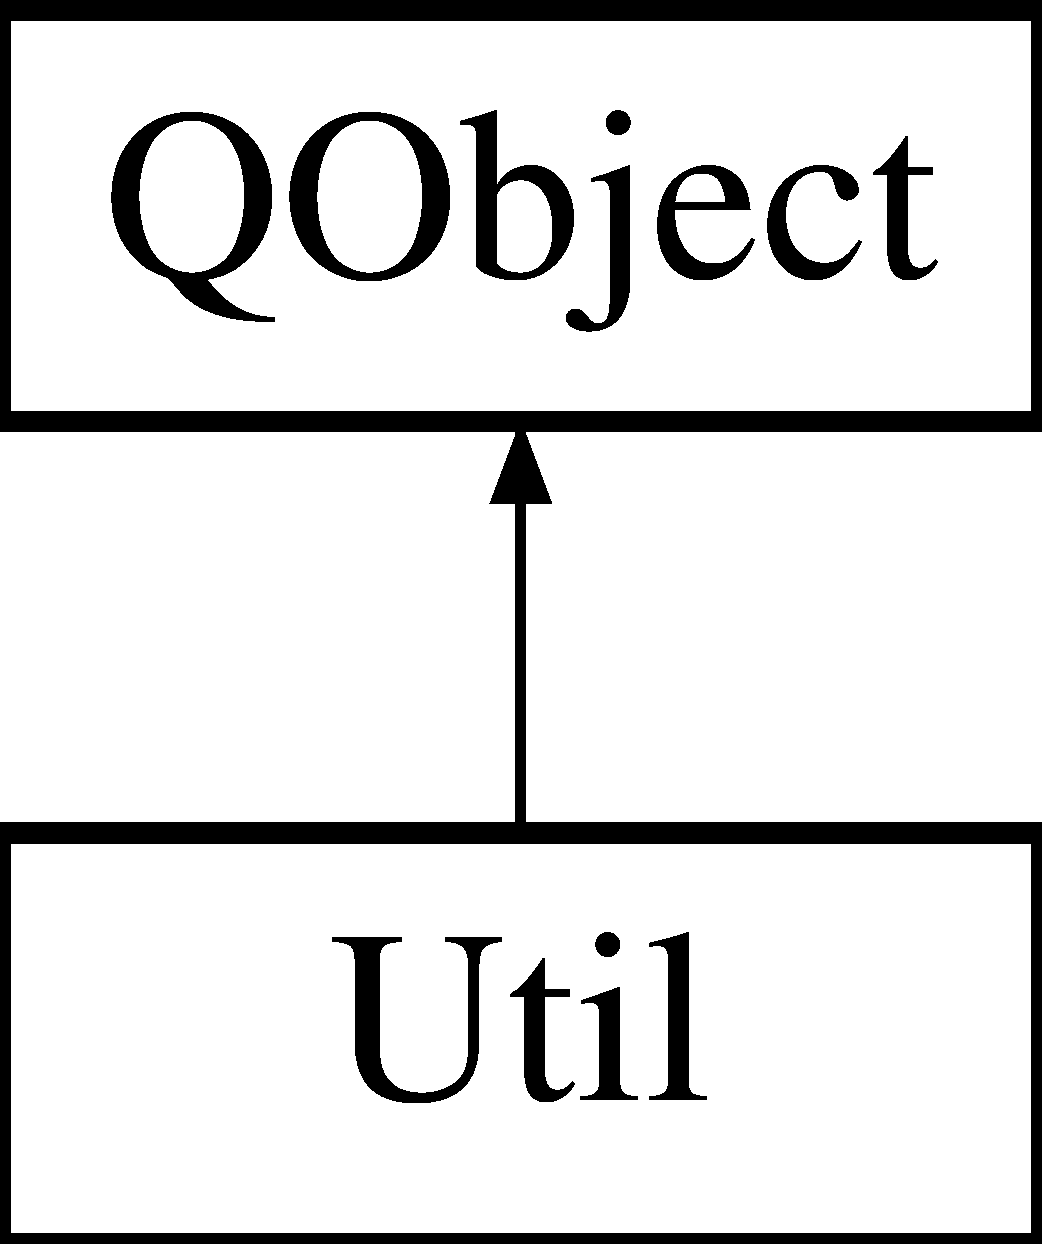
\includegraphics[height=2.000000cm]{classUtil}
\end{center}
\end{figure}
\subsection*{Public Member Functions}
\begin{DoxyCompactItemize}
\item 
\hypertarget{classUtil_a500a30db3919321f09834b01196a8ce6}{{\bfseries Util} (Q\-Object $\ast$parent=nullptr)}\label{classUtil_a500a30db3919321f09834b01196a8ce6}

\item 
int \hyperlink{classUtil_a1a4d673faba2294b89dbff114011703f}{hash\-Password} (Q\-String password)
\item 
bool \hyperlink{classUtil_a6f479a120988b9283e7198bae0555ece}{check\-Password} (Q\-String password)
\end{DoxyCompactItemize}


\subsection{Member Function Documentation}
\hypertarget{classUtil_a6f479a120988b9283e7198bae0555ece}{\index{Util@{Util}!check\-Password@{check\-Password}}
\index{check\-Password@{check\-Password}!Util@{Util}}
\subsubsection[{check\-Password}]{\setlength{\rightskip}{0pt plus 5cm}bool Util\-::check\-Password (
\begin{DoxyParamCaption}
\item[{Q\-String}]{password}
\end{DoxyParamCaption}
)}}\label{classUtil_a6f479a120988b9283e7198bae0555ece}
Checks if a password is valid, of size at least 4 and have special chars /return True if valid, false otherwise. \hypertarget{classUtil_a1a4d673faba2294b89dbff114011703f}{\index{Util@{Util}!hash\-Password@{hash\-Password}}
\index{hash\-Password@{hash\-Password}!Util@{Util}}
\subsubsection[{hash\-Password}]{\setlength{\rightskip}{0pt plus 5cm}int Util\-::hash\-Password (
\begin{DoxyParamCaption}
\item[{Q\-String}]{password}
\end{DoxyParamCaption}
)}}\label{classUtil_a1a4d673faba2294b89dbff114011703f}
Hashes a password using a hashfunction /return Hashed password as int 

The documentation for this class was generated from the following files\-:\begin{DoxyCompactItemize}
\item 
accounts-\/and-\/framework/util.\-h\item 
accounts-\/and-\/framework/util.\-cpp\end{DoxyCompactItemize}

\hypertarget{classVirusLarge}{\section{Virus\-Large Class Reference}
\label{classVirusLarge}\index{Virus\-Large@{Virus\-Large}}
}
Inheritance diagram for Virus\-Large\-:\begin{figure}[H]
\begin{center}
\leavevmode
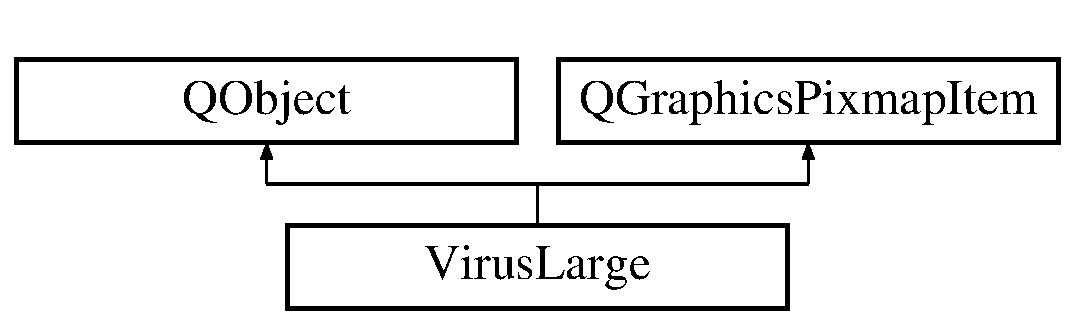
\includegraphics[height=2.000000cm]{classVirusLarge}
\end{center}
\end{figure}
\subsection*{Public Slots}
\begin{DoxyCompactItemize}
\item 
void \hyperlink{classVirusLarge_a1867409aa12e3854510355692590e6b8}{update} ()
\end{DoxyCompactItemize}
\subsection*{Signals}
\begin{DoxyCompactItemize}
\item 
\hypertarget{classVirusLarge_aaca3750970743cfbacd43a8a22db4686}{void {\bfseries collision} ()}\label{classVirusLarge_aaca3750970743cfbacd43a8a22db4686}

\item 
\hypertarget{classVirusLarge_a01036cf40eff4e17626f23137934ca6d}{void {\bfseries failure} ()}\label{classVirusLarge_a01036cf40eff4e17626f23137934ca6d}

\end{DoxyCompactItemize}
\subsection*{Public Member Functions}
\begin{DoxyCompactItemize}
\item 
\hypertarget{classVirusLarge_a5948e319e9f2caf7823fee9d2966a793}{{\bfseries Virus\-Large} (Q\-Object $\ast$parent=nullptr, int level\-Speed=50)}\label{classVirusLarge_a5948e319e9f2caf7823fee9d2966a793}

\item 
void \hyperlink{classVirusLarge_a6fc4f92c9da1c5e28c1947614d07e106}{collided\-With\-Syringe} ()
\item 
void \hyperlink{classVirusLarge_a3f782b098d766045c3741b5ba3af412b}{user\-Failed} ()
\end{DoxyCompactItemize}
\subsection*{Public Attributes}
\begin{DoxyCompactItemize}
\item 
\hypertarget{classVirusLarge_a248ecb0626b53adca976924bfe8db885}{Q\-String {\bfseries picture\-Path} = \char`\"{}\-:/game1images/virus-\/green.\-png\char`\"{}}\label{classVirusLarge_a248ecb0626b53adca976924bfe8db885}

\item 
\hypertarget{classVirusLarge_a55db6edef36b3076075a58c3da047eca}{Q\-String {\bfseries smashed\-Pic\-Path} = \char`\"{}\-:/game1images/mike.\-png\char`\"{}}\label{classVirusLarge_a55db6edef36b3076075a58c3da047eca}

\item 
\hypertarget{classVirusLarge_a289b9bee5206025dddea768e51a044de}{bool {\bfseries smashed} = false}\label{classVirusLarge_a289b9bee5206025dddea768e51a044de}

\item 
\hypertarget{classVirusLarge_ab5359e58ba24e94e01b124b0c0965047}{int {\bfseries x}}\label{classVirusLarge_ab5359e58ba24e94e01b124b0c0965047}

\item 
\hypertarget{classVirusLarge_aa84d4112904daf3e1b0eed10609b22f2}{int {\bfseries y}}\label{classVirusLarge_aa84d4112904daf3e1b0eed10609b22f2}

\item 
\hypertarget{classVirusLarge_aa0e103b493a8e1521f14bde2c32b143b}{int {\bfseries virus\-Type} = 1}\label{classVirusLarge_aa0e103b493a8e1521f14bde2c32b143b}

\item 
\hypertarget{classVirusLarge_adee2818d276e71e75edc62d4d8cbcb21}{int {\bfseries virus\-Score} = 0}\label{classVirusLarge_adee2818d276e71e75edc62d4d8cbcb21}

\item 
\hypertarget{classVirusLarge_addab58ac66d2575d66afb3c764c12886}{int {\bfseries timer\-Speed} = 50}\label{classVirusLarge_addab58ac66d2575d66afb3c764c12886}

\item 
\hypertarget{classVirusLarge_a7de3fc5029cfa419e250cd819c3eb09e}{Q\-Timer $\ast$ {\bfseries timer}}\label{classVirusLarge_a7de3fc5029cfa419e250cd819c3eb09e}

\end{DoxyCompactItemize}


\subsection{Member Function Documentation}
\hypertarget{classVirusLarge_a6fc4f92c9da1c5e28c1947614d07e106}{\index{Virus\-Large@{Virus\-Large}!collided\-With\-Syringe@{collided\-With\-Syringe}}
\index{collided\-With\-Syringe@{collided\-With\-Syringe}!VirusLarge@{Virus\-Large}}
\subsubsection[{collided\-With\-Syringe}]{\setlength{\rightskip}{0pt plus 5cm}void Virus\-Large\-::collided\-With\-Syringe (
\begin{DoxyParamCaption}
{}
\end{DoxyParamCaption}
)}}\label{classVirusLarge_a6fc4f92c9da1c5e28c1947614d07e106}
A function that emits a signal whenever a collision happens with a virus \hypertarget{classVirusLarge_a1867409aa12e3854510355692590e6b8}{\index{Virus\-Large@{Virus\-Large}!update@{update}}
\index{update@{update}!VirusLarge@{Virus\-Large}}
\subsubsection[{update}]{\setlength{\rightskip}{0pt plus 5cm}void Virus\-Large\-::update (
\begin{DoxyParamCaption}
{}
\end{DoxyParamCaption}
)\hspace{0.3cm}{\ttfamily [slot]}}}\label{classVirusLarge_a1867409aa12e3854510355692590e6b8}
A function that updates the coordinates of a virus \hypertarget{classVirusLarge_a3f782b098d766045c3741b5ba3af412b}{\index{Virus\-Large@{Virus\-Large}!user\-Failed@{user\-Failed}}
\index{user\-Failed@{user\-Failed}!VirusLarge@{Virus\-Large}}
\subsubsection[{user\-Failed}]{\setlength{\rightskip}{0pt plus 5cm}void Virus\-Large\-::user\-Failed (
\begin{DoxyParamCaption}
{}
\end{DoxyParamCaption}
)}}\label{classVirusLarge_a3f782b098d766045c3741b5ba3af412b}
emit a signal whenever the syringe fails to hit the Virus -\/ Game Over! 

The documentation for this class was generated from the following files\-:\begin{DoxyCompactItemize}
\item 
game1-\/kill-\/covid-\/19/viruslarge.\-h\item 
game1-\/kill-\/covid-\/19/viruslarge.\-cpp\end{DoxyCompactItemize}

\hypertarget{classWelcomeWindow}{\section{Welcome\-Window Class Reference}
\label{classWelcomeWindow}\index{Welcome\-Window@{Welcome\-Window}}
}
Inheritance diagram for Welcome\-Window\-:\begin{figure}[H]
\begin{center}
\leavevmode
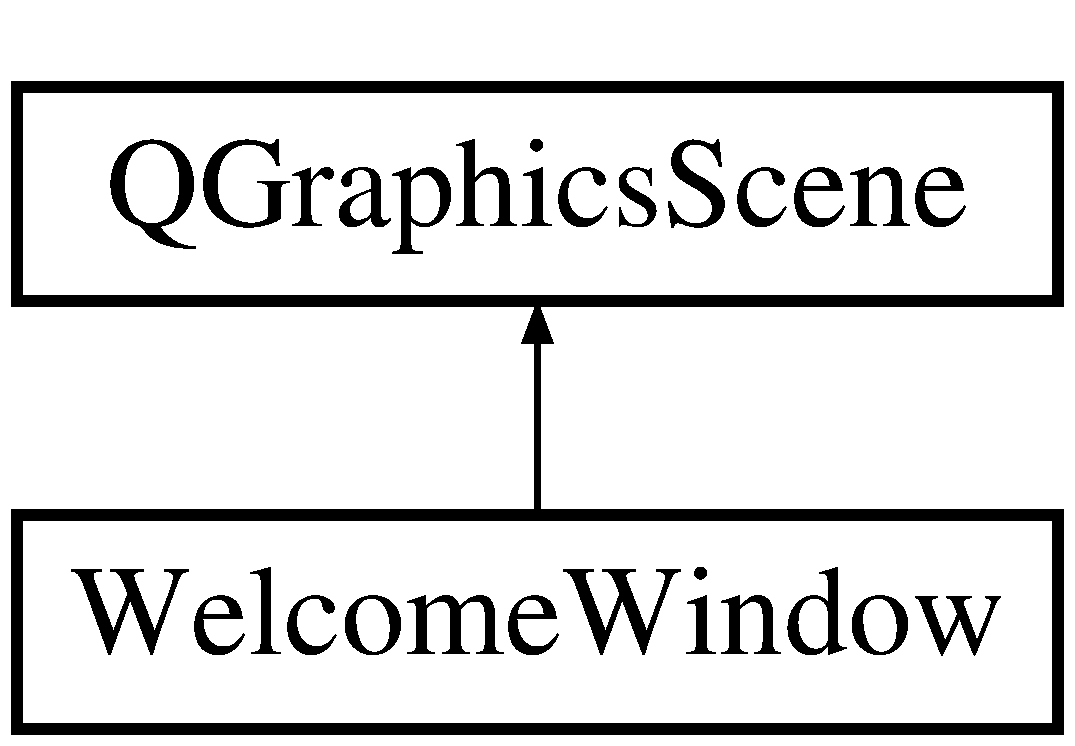
\includegraphics[height=2.000000cm]{classWelcomeWindow}
\end{center}
\end{figure}
\subsection*{Public Member Functions}
\begin{DoxyCompactItemize}
\item 
\hypertarget{classWelcomeWindow_a2f8c0bb7ffe56a2a27f5fd3d43518c39}{{\bfseries Welcome\-Window} (Q\-Object $\ast$parent=nullptr)}\label{classWelcomeWindow_a2f8c0bb7ffe56a2a27f5fd3d43518c39}

\item 
void \hyperlink{classWelcomeWindow_ad367652cb1e5ad31409d458f3bafb043}{fix\-Pixmap\-Items} ()
\item 
void \hyperlink{classWelcomeWindow_a0f4ffd1e10871df8d44702efb6566a86}{fix\-Widgets} ()
\item 
void \hyperlink{classWelcomeWindow_a92c93c12c2de7f24ee6fea83b099a548}{fix\-Labels} ()
\item 
void \hyperlink{classWelcomeWindow_a9bd72538fefc87e5cad3a5931529c868}{fill\-Scene} ()
\item 
void \hyperlink{classWelcomeWindow_a1fe8b2a01a787dd0f7f7da0c3bf2f309}{check\-Bday} ()
\item 
void \hyperlink{classWelcomeWindow_aa2525422faa9826e5719a81bdbf7c197}{update\-Profile\-Pic} ()
\item 
void \hyperlink{classWelcomeWindow_a7907ba084c2f59b8be82086cc5a48093}{update\-Scores} ()
\item 
void \hyperlink{classWelcomeWindow_aaa915a1d2bffe88b815d0c8fcdcc7734}{clean\-Page} ()
\end{DoxyCompactItemize}
\subsection*{Public Attributes}
\begin{DoxyCompactItemize}
\item 
\hypertarget{classWelcomeWindow_adf9d45bef2656e20de1f0fda3da6de95}{\hyperlink{classUser}{User} $\ast$ {\bfseries cur\-User} = N\-U\-L\-L}\label{classWelcomeWindow_adf9d45bef2656e20de1f0fda3da6de95}

\item 
\hypertarget{classWelcomeWindow_ab8507dc4fbc7ece52dcbd9607840b308}{\hyperlink{classJson}{Json} {\bfseries json}}\label{classWelcomeWindow_ab8507dc4fbc7ece52dcbd9607840b308}

\item 
\hypertarget{classWelcomeWindow_a3a8a6bdf275bf15135afdcda58e404b9}{Q\-Label $\ast$ {\bfseries hello\-Label}}\label{classWelcomeWindow_a3a8a6bdf275bf15135afdcda58e404b9}

\item 
\hypertarget{classWelcomeWindow_a5c7f6fed6aa596e7136b2d2e920225fa}{Q\-Label $\ast$ {\bfseries happy\-Birthday}}\label{classWelcomeWindow_a5c7f6fed6aa596e7136b2d2e920225fa}

\item 
\hypertarget{classWelcomeWindow_a763e1ed9bde558a472e47e330d5d98a1}{Q\-Graphics\-Pixmap\-Item $\ast$ {\bfseries game1\-Pic}}\label{classWelcomeWindow_a763e1ed9bde558a472e47e330d5d98a1}

\item 
\hypertarget{classWelcomeWindow_affd78ea126d680bf6a1aed66b0c73bcd}{Q\-Graphics\-Pixmap\-Item $\ast$ {\bfseries game2\-Pic}}\label{classWelcomeWindow_affd78ea126d680bf6a1aed66b0c73bcd}

\item 
\hypertarget{classWelcomeWindow_a77b486a7541f2731c874dff15b0500ef}{Q\-Graphics\-Pixmap\-Item $\ast$ {\bfseries profile\-Picture}}\label{classWelcomeWindow_a77b486a7541f2731c874dff15b0500ef}

\item 
\hypertarget{classWelcomeWindow_ac74aeed412d90ec3800659a413c5b691}{Q\-Push\-Button $\ast$ {\bfseries game1\-Button}}\label{classWelcomeWindow_ac74aeed412d90ec3800659a413c5b691}

\item 
\hypertarget{classWelcomeWindow_a67cc4d6dee956184e049eacbaa6fd3ca}{Q\-Push\-Button $\ast$ {\bfseries game2\-Button}}\label{classWelcomeWindow_a67cc4d6dee956184e049eacbaa6fd3ca}

\item 
\hypertarget{classWelcomeWindow_a6cd624e2c8d6b00551ada959b862a449}{Q\-Push\-Button $\ast$ {\bfseries home\-Button}}\label{classWelcomeWindow_a6cd624e2c8d6b00551ada959b862a449}

\item 
\hypertarget{classWelcomeWindow_a4f78aa4ec4752e4a51fc25886062b06c}{Q\-Label $\ast$ {\bfseries game1\-Scores}}\label{classWelcomeWindow_a4f78aa4ec4752e4a51fc25886062b06c}

\item 
\hypertarget{classWelcomeWindow_af36a2fff96d012c90785fef512f02885}{Q\-Label $\ast$ {\bfseries game2\-Scores}}\label{classWelcomeWindow_af36a2fff96d012c90785fef512f02885}

\end{DoxyCompactItemize}


\subsection{Member Function Documentation}
\hypertarget{classWelcomeWindow_a1fe8b2a01a787dd0f7f7da0c3bf2f309}{\index{Welcome\-Window@{Welcome\-Window}!check\-Bday@{check\-Bday}}
\index{check\-Bday@{check\-Bday}!WelcomeWindow@{Welcome\-Window}}
\subsubsection[{check\-Bday}]{\setlength{\rightskip}{0pt plus 5cm}void Welcome\-Window\-::check\-Bday (
\begin{DoxyParamCaption}
{}
\end{DoxyParamCaption}
)}}\label{classWelcomeWindow_a1fe8b2a01a787dd0f7f7da0c3bf2f309}
checks if its the current user's birthday. if so, displays a happy birthday message \hypertarget{classWelcomeWindow_aaa915a1d2bffe88b815d0c8fcdcc7734}{\index{Welcome\-Window@{Welcome\-Window}!clean\-Page@{clean\-Page}}
\index{clean\-Page@{clean\-Page}!WelcomeWindow@{Welcome\-Window}}
\subsubsection[{clean\-Page}]{\setlength{\rightskip}{0pt plus 5cm}void Welcome\-Window\-::clean\-Page (
\begin{DoxyParamCaption}
{}
\end{DoxyParamCaption}
)}}\label{classWelcomeWindow_aaa915a1d2bffe88b815d0c8fcdcc7734}
Called when we need to go to the maingview Cleans all widgets in order to prepare for another user to login/signup \hypertarget{classWelcomeWindow_a9bd72538fefc87e5cad3a5931529c868}{\index{Welcome\-Window@{Welcome\-Window}!fill\-Scene@{fill\-Scene}}
\index{fill\-Scene@{fill\-Scene}!WelcomeWindow@{Welcome\-Window}}
\subsubsection[{fill\-Scene}]{\setlength{\rightskip}{0pt plus 5cm}void Welcome\-Window\-::fill\-Scene (
\begin{DoxyParamCaption}
{}
\end{DoxyParamCaption}
)}}\label{classWelcomeWindow_a9bd72538fefc87e5cad3a5931529c868}
Function Used to fill the Scene -\/ For readability \hypertarget{classWelcomeWindow_a92c93c12c2de7f24ee6fea83b099a548}{\index{Welcome\-Window@{Welcome\-Window}!fix\-Labels@{fix\-Labels}}
\index{fix\-Labels@{fix\-Labels}!WelcomeWindow@{Welcome\-Window}}
\subsubsection[{fix\-Labels}]{\setlength{\rightskip}{0pt plus 5cm}void Welcome\-Window\-::fix\-Labels (
\begin{DoxyParamCaption}
{}
\end{DoxyParamCaption}
)}}\label{classWelcomeWindow_a92c93c12c2de7f24ee6fea83b099a548}
Function used to fix Labels -\/ For readability \hypertarget{classWelcomeWindow_ad367652cb1e5ad31409d458f3bafb043}{\index{Welcome\-Window@{Welcome\-Window}!fix\-Pixmap\-Items@{fix\-Pixmap\-Items}}
\index{fix\-Pixmap\-Items@{fix\-Pixmap\-Items}!WelcomeWindow@{Welcome\-Window}}
\subsubsection[{fix\-Pixmap\-Items}]{\setlength{\rightskip}{0pt plus 5cm}void Welcome\-Window\-::fix\-Pixmap\-Items (
\begin{DoxyParamCaption}
{}
\end{DoxyParamCaption}
)}}\label{classWelcomeWindow_ad367652cb1e5ad31409d458f3bafb043}
Sets the icons of the games in their corresponding place on the scene \hypertarget{classWelcomeWindow_a0f4ffd1e10871df8d44702efb6566a86}{\index{Welcome\-Window@{Welcome\-Window}!fix\-Widgets@{fix\-Widgets}}
\index{fix\-Widgets@{fix\-Widgets}!WelcomeWindow@{Welcome\-Window}}
\subsubsection[{fix\-Widgets}]{\setlength{\rightskip}{0pt plus 5cm}void Welcome\-Window\-::fix\-Widgets (
\begin{DoxyParamCaption}
{}
\end{DoxyParamCaption}
)}}\label{classWelcomeWindow_a0f4ffd1e10871df8d44702efb6566a86}
Sets the geometry of the widgets \hypertarget{classWelcomeWindow_aa2525422faa9826e5719a81bdbf7c197}{\index{Welcome\-Window@{Welcome\-Window}!update\-Profile\-Pic@{update\-Profile\-Pic}}
\index{update\-Profile\-Pic@{update\-Profile\-Pic}!WelcomeWindow@{Welcome\-Window}}
\subsubsection[{update\-Profile\-Pic}]{\setlength{\rightskip}{0pt plus 5cm}void Welcome\-Window\-::update\-Profile\-Pic (
\begin{DoxyParamCaption}
{}
\end{DoxyParamCaption}
)}}\label{classWelcomeWindow_aa2525422faa9826e5719a81bdbf7c197}
Decodes a user's profile picture from a Q\-Json\-Value into a Q\-Pixmap sets the Pixmap p to the corresponding profile pic location on the scene \hypertarget{classWelcomeWindow_a7907ba084c2f59b8be82086cc5a48093}{\index{Welcome\-Window@{Welcome\-Window}!update\-Scores@{update\-Scores}}
\index{update\-Scores@{update\-Scores}!WelcomeWindow@{Welcome\-Window}}
\subsubsection[{update\-Scores}]{\setlength{\rightskip}{0pt plus 5cm}void Welcome\-Window\-::update\-Scores (
\begin{DoxyParamCaption}
{}
\end{DoxyParamCaption}
)}}\label{classWelcomeWindow_a7907ba084c2f59b8be82086cc5a48093}
Displays a user's scores to the scene for each corresponding game 

The documentation for this class was generated from the following files\-:\begin{DoxyCompactItemize}
\item 
accounts-\/and-\/framework/welcomewindow.\-h\item 
accounts-\/and-\/framework/welcomewindow.\-cpp\end{DoxyCompactItemize}

%--- End generated contents ---

% Index
\newpage
\phantomsection
\addcontentsline{toc}{chapter}{Index}
\printindex

\end{document}
